% Archivo: 4_results_and_discussion.tex
\section{Resultados y Discusión}

\subsection{Caminos aleatorios}

Las simulaciones de los caminos aleatorios validan con alta precisión la predicción analítica. Los ajustes lineales de $\langle r^2 \rangle$ frente al tiempo muestran proporcionalidad cercana a la unidad, confirmando que la varianza de la posición crece linealmente sin importar la dimensionalidad (1D, 2D o 3D) o la geometría (coordenadas cartesianas o polares), siempre que la distancia total recorrida en cada paso sea igual en todos los casos.

\subsubsection{Caminata Aleatoria en 1D}

Como se observa en la Figura \ref{fig:rw_1d}, las trayectorias individuales muestran la típica divergencia estocástica desde el origen a medida que avanza el tiempo.

\begin{figure}[htbp]
    \centering
    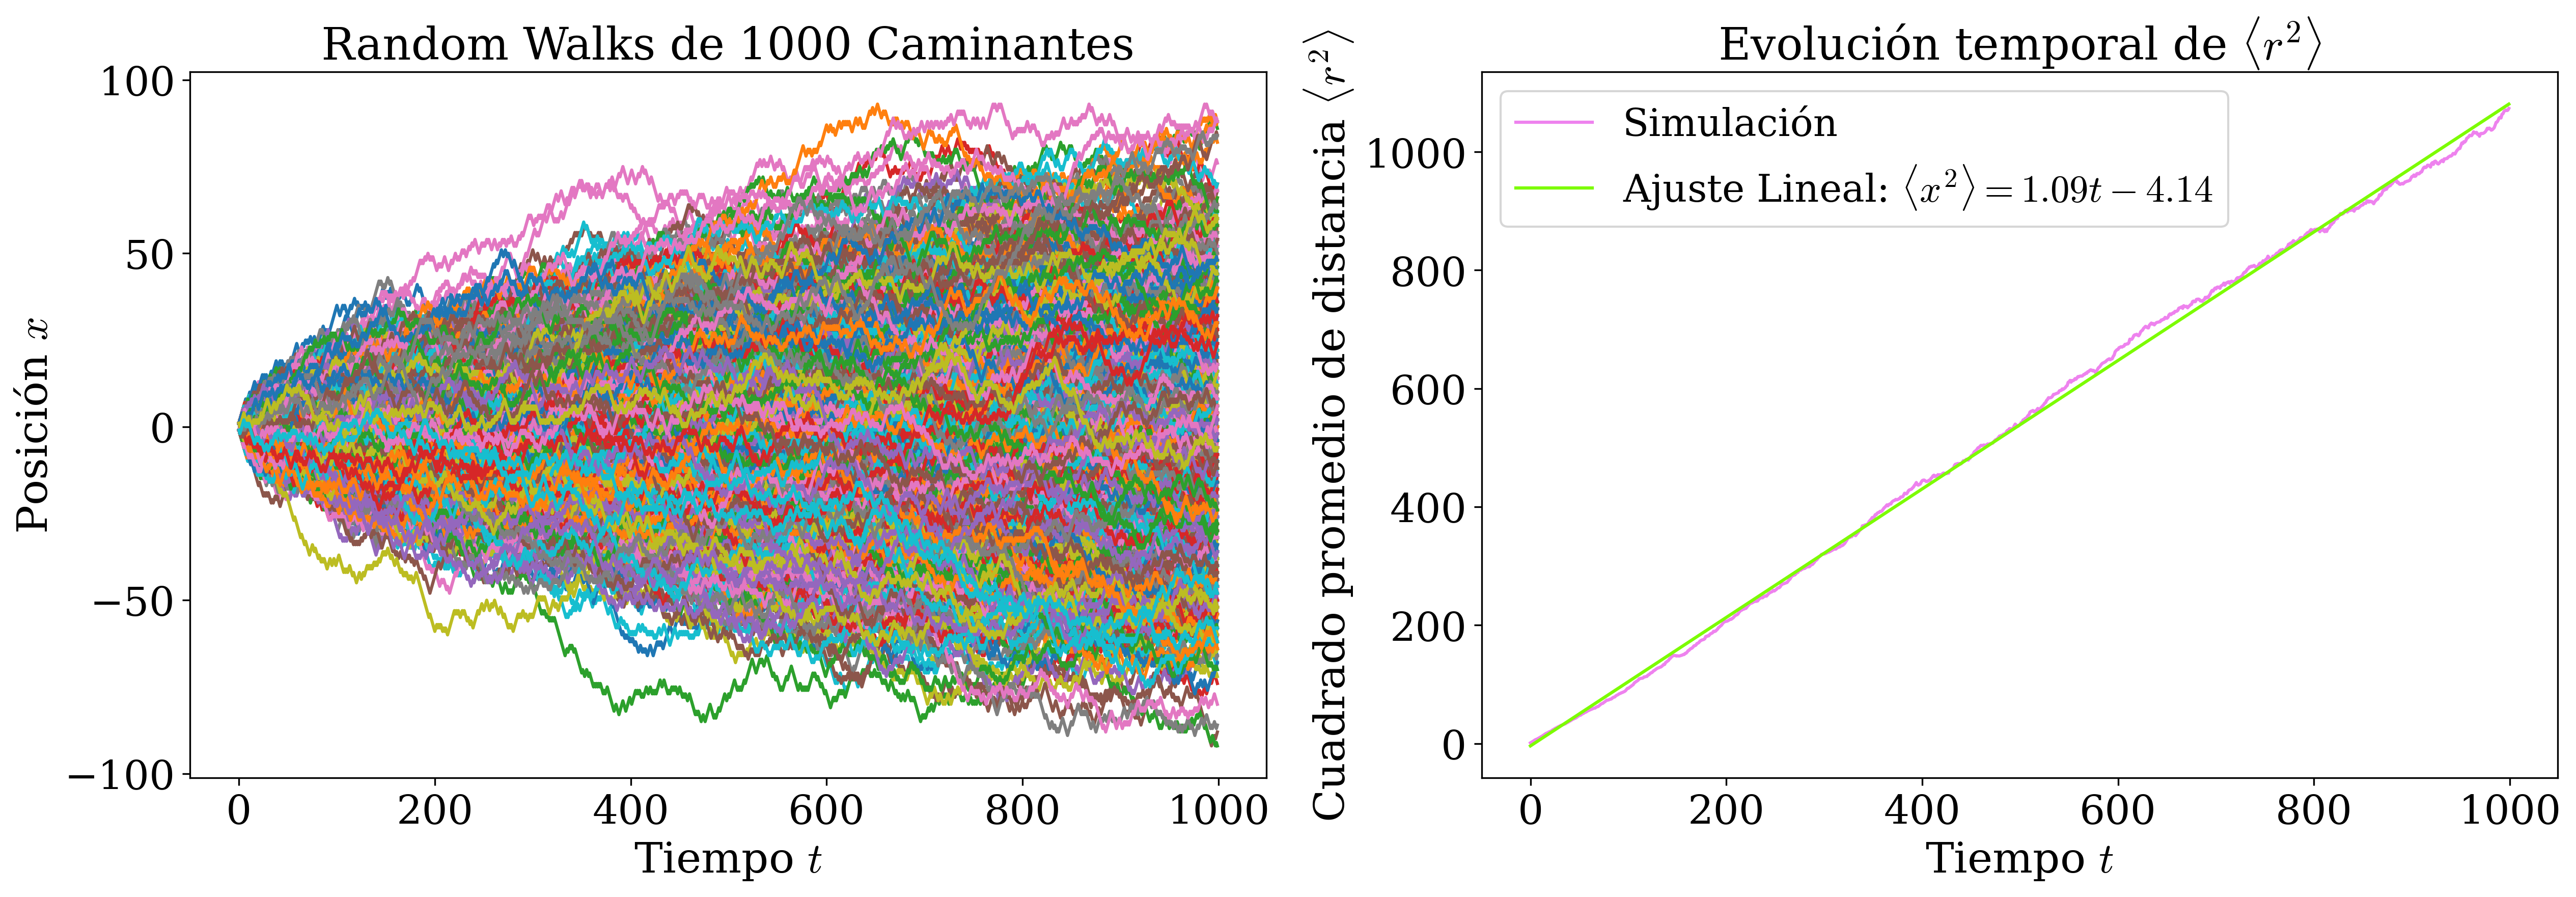
\includegraphics[width=\textwidth]{figures_tex/rw_1d.png}
    \caption{A la izquierda: Posición $x$ frente al tiempo $t$ para $N=1000$ caminantes en 1D. A la derecha: Evolución temporal del desplazamiento cuadrático medio $\langle r^2 \rangle$ con su respectivo ajuste lineal.}
    \label{fig:rw_1d}
\end{figure}

La simulación para $N = 1000$ caminantes a lo largo de $t = 1000$ pasos revela una dispersión simétrica respecto al origen ($x=0$), haciendo patente la relación $\langle x_N \rangle = 0$. Por su parte, la linealidad estricta observada en la evolución de $\langle r^2 \rangle$ confirma empíricamente la ley de difusión de Fick para un movimiento browniano estándar. La pendiente de $1.09$ es una aproximación numérica al coeficiente teórico esperado según \ref{eq:r2}.

\subsubsection{Caminata Aleatoria en 2D: Coordenadas Cartesianas y Polares}

Para el caso bidimensional, se contrastaron dos enfoques de muestreo espacial: uno basado en incrementos cartesianos y otro en coordenadas polares. En ambos casos, se emplearon un total de $N=1000$ caminantes. Se puede acceder a la trayectoria de uno de los caminante en \href{https://www.youtube.com/watch_videos?video_ids=GMyH0yJqf_M,dOK2JVeqVpE}{YouTube}.

\begin{figure}[htbp]
    \centering
    \begin{minipage}{0.54\textwidth}
        \centering
        \href{https://youtu.be/GMyH0yJqf_M?list=PLYDzV8MgIoON7YU9Pd_x0HvjzlLKixw87}{
        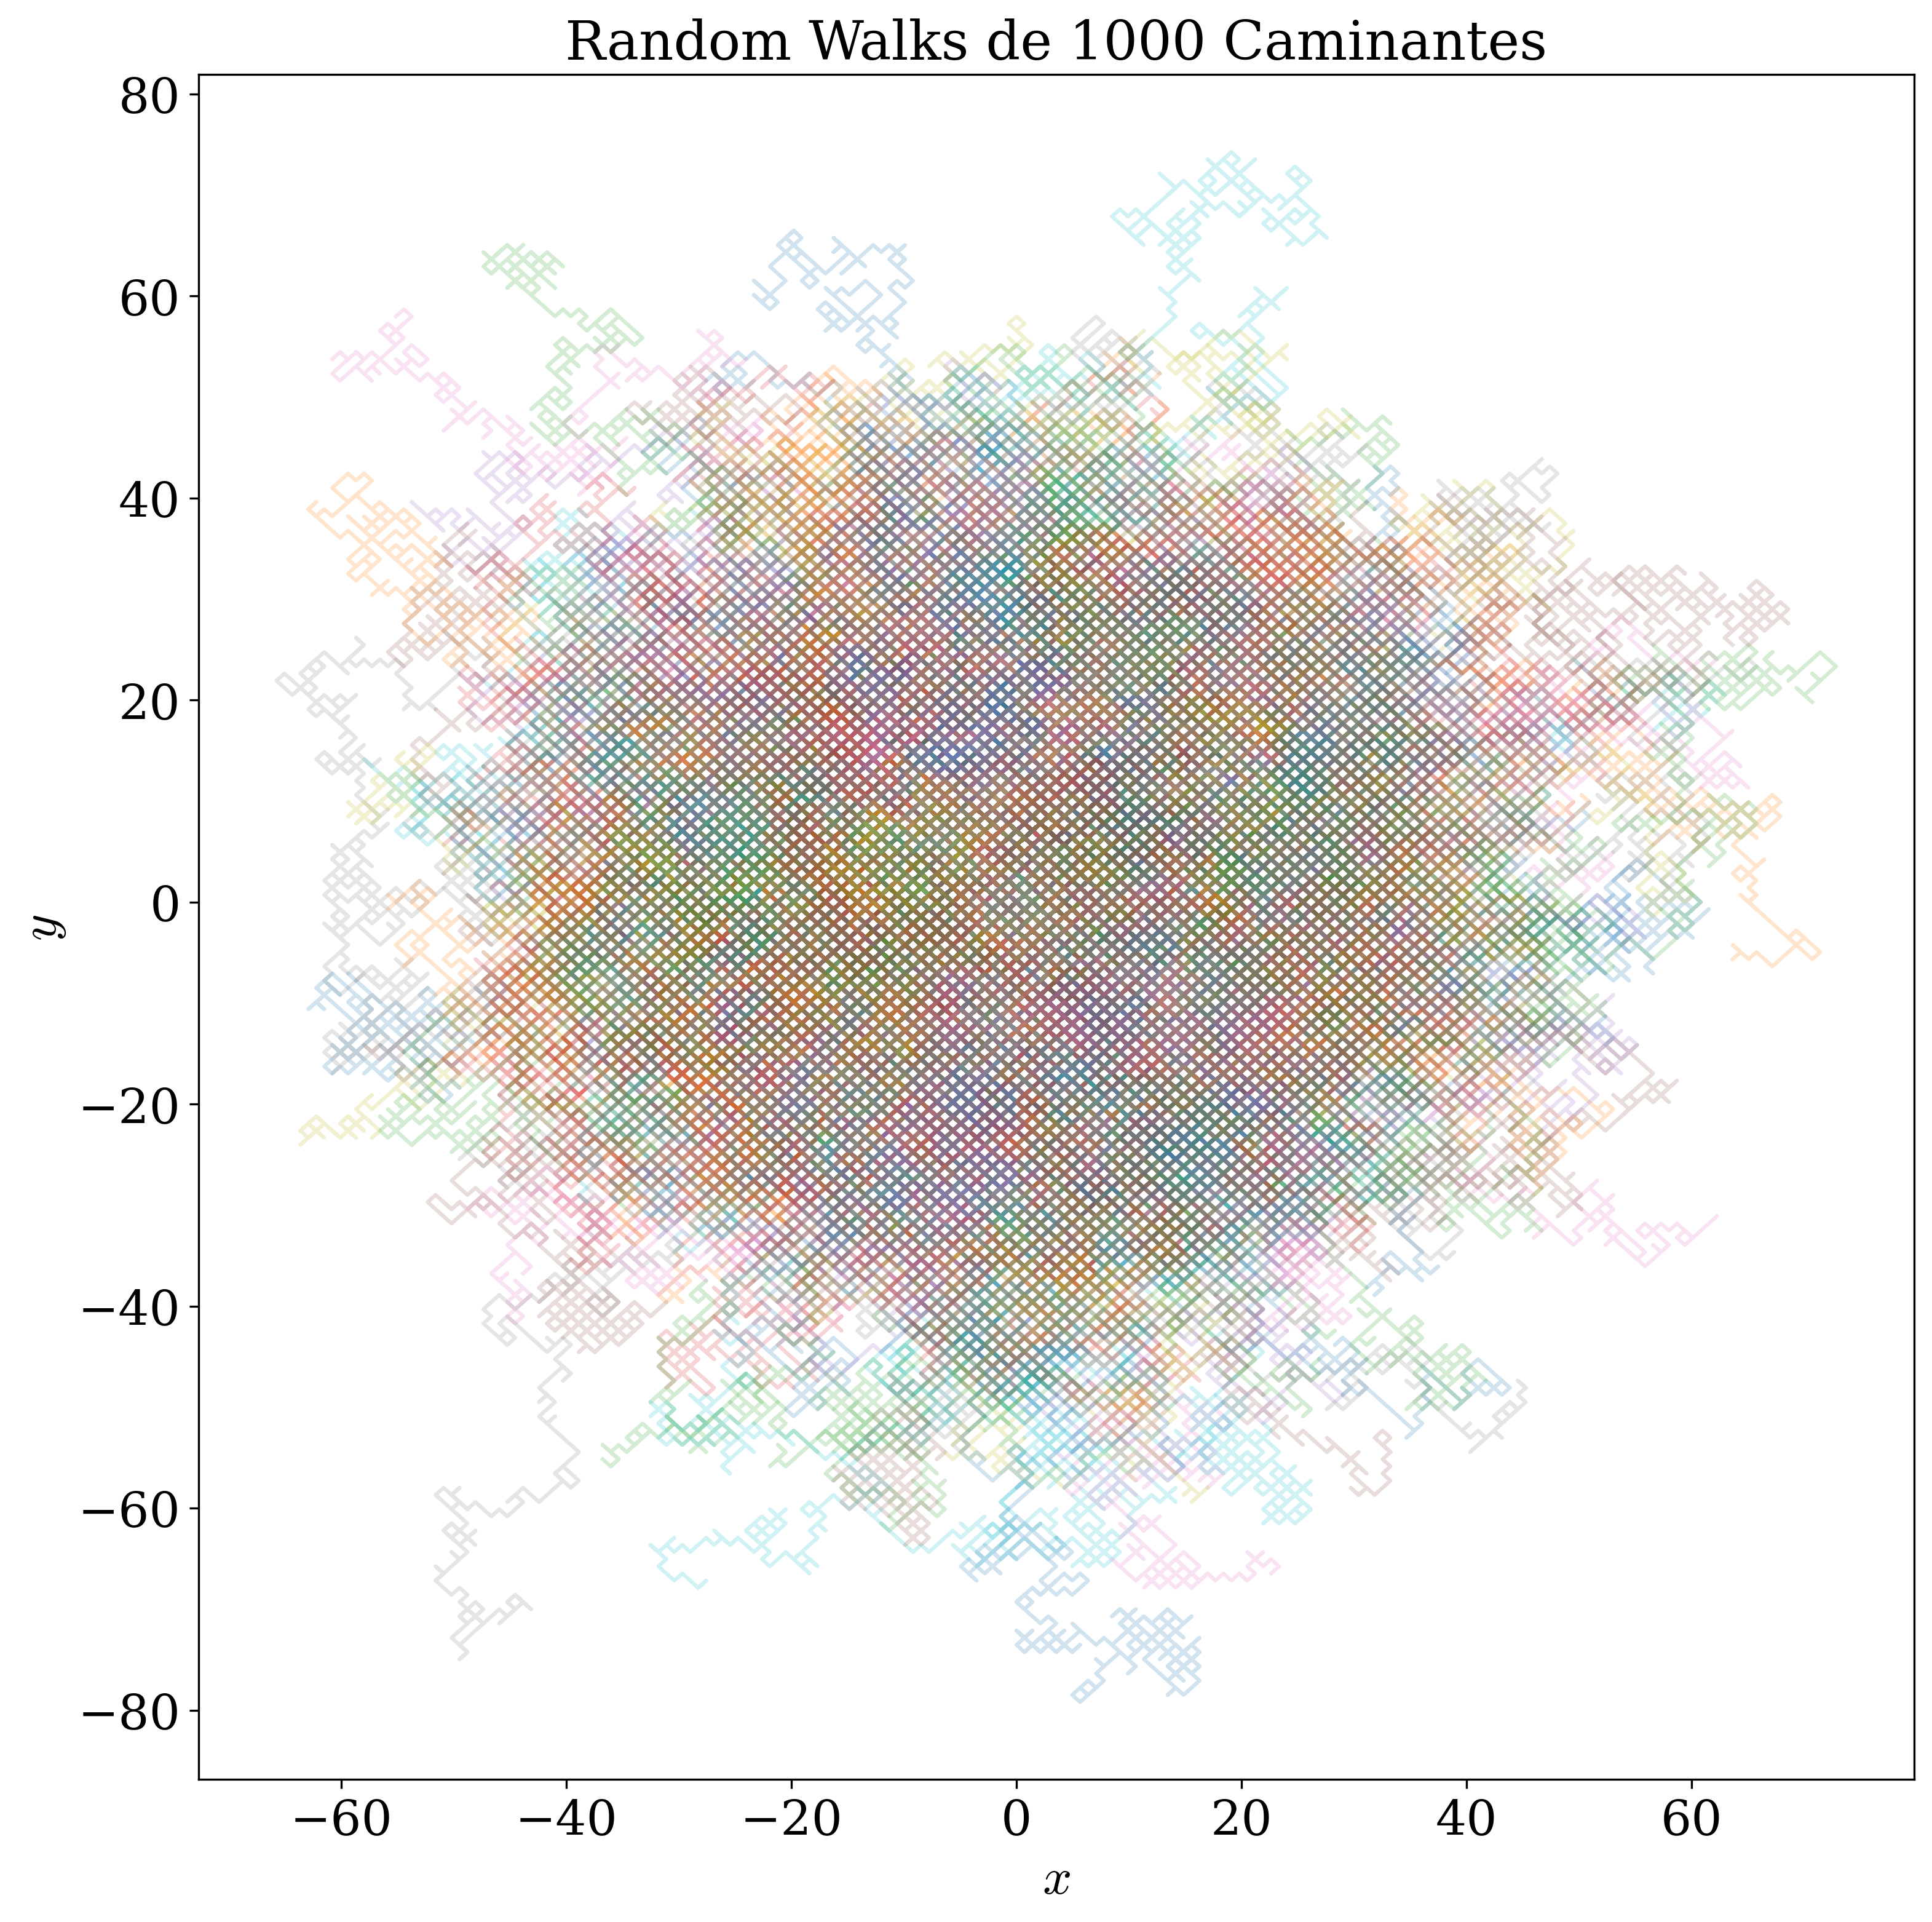
\includegraphics[width=\textwidth]{figures_tex/rw_2d_cart.png}}
        \caption{Trayectorias en el plano $xy$.}
        \label{fig:rw_2d_cart}
    \end{minipage}\hfill
    \begin{minipage}{0.44\textwidth}
        \centering
        \href{https://youtu.be/dOK2JVeqVpE?list=PLYDzV8MgIoON7YU9Pd_x0HvjzlLKixw87}{
        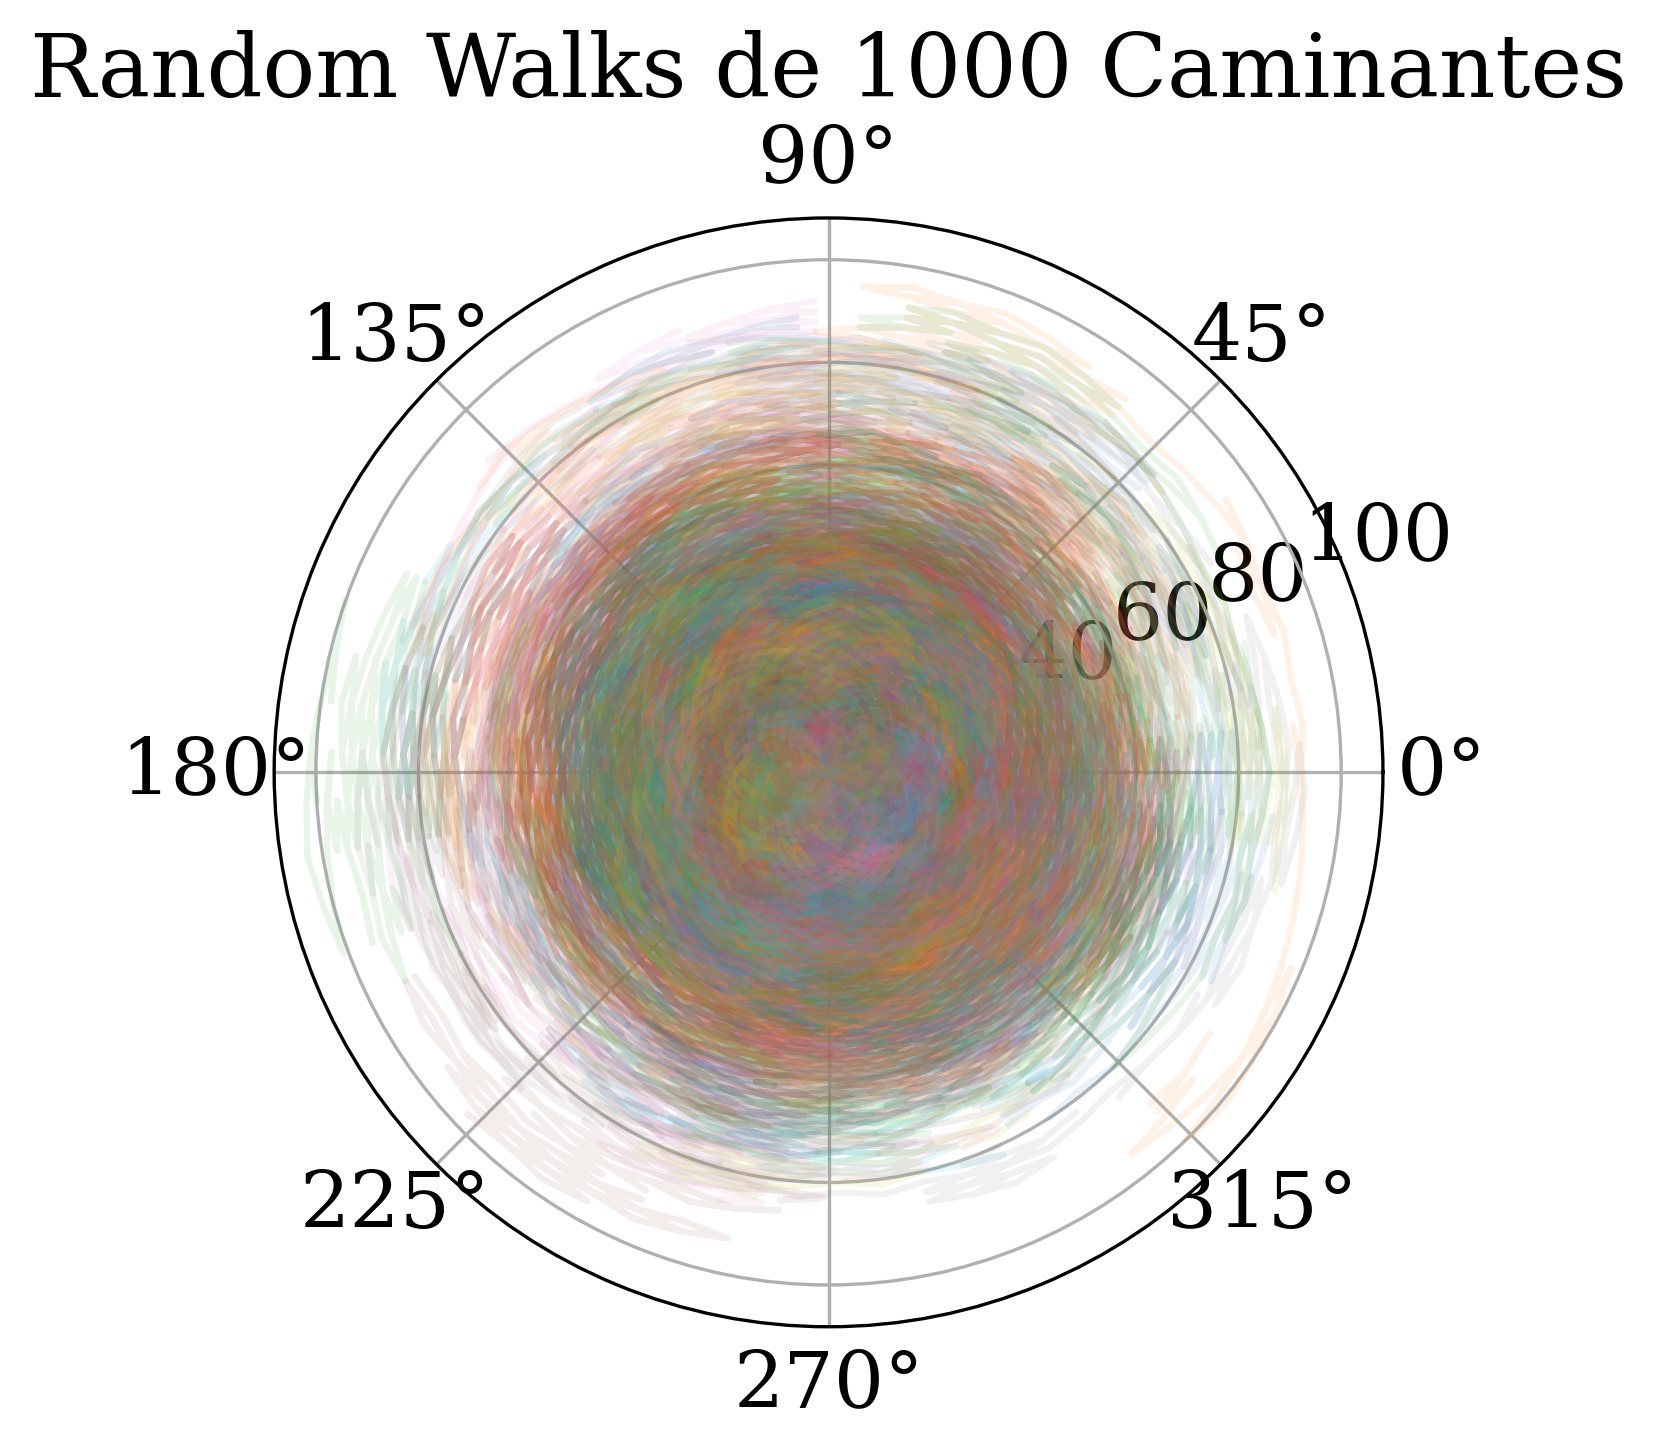
\includegraphics[width=\textwidth]{figures_tex/rw_2d_polar.png}}
        \caption{Trayectorias en plano polar.}
        \label{fig:rw_2d_polar}
    \end{minipage}


\end{figure}

\begin{figure}[htbp]
    \centering
    \begin{minipage}{0.48\textwidth}
        \centering
        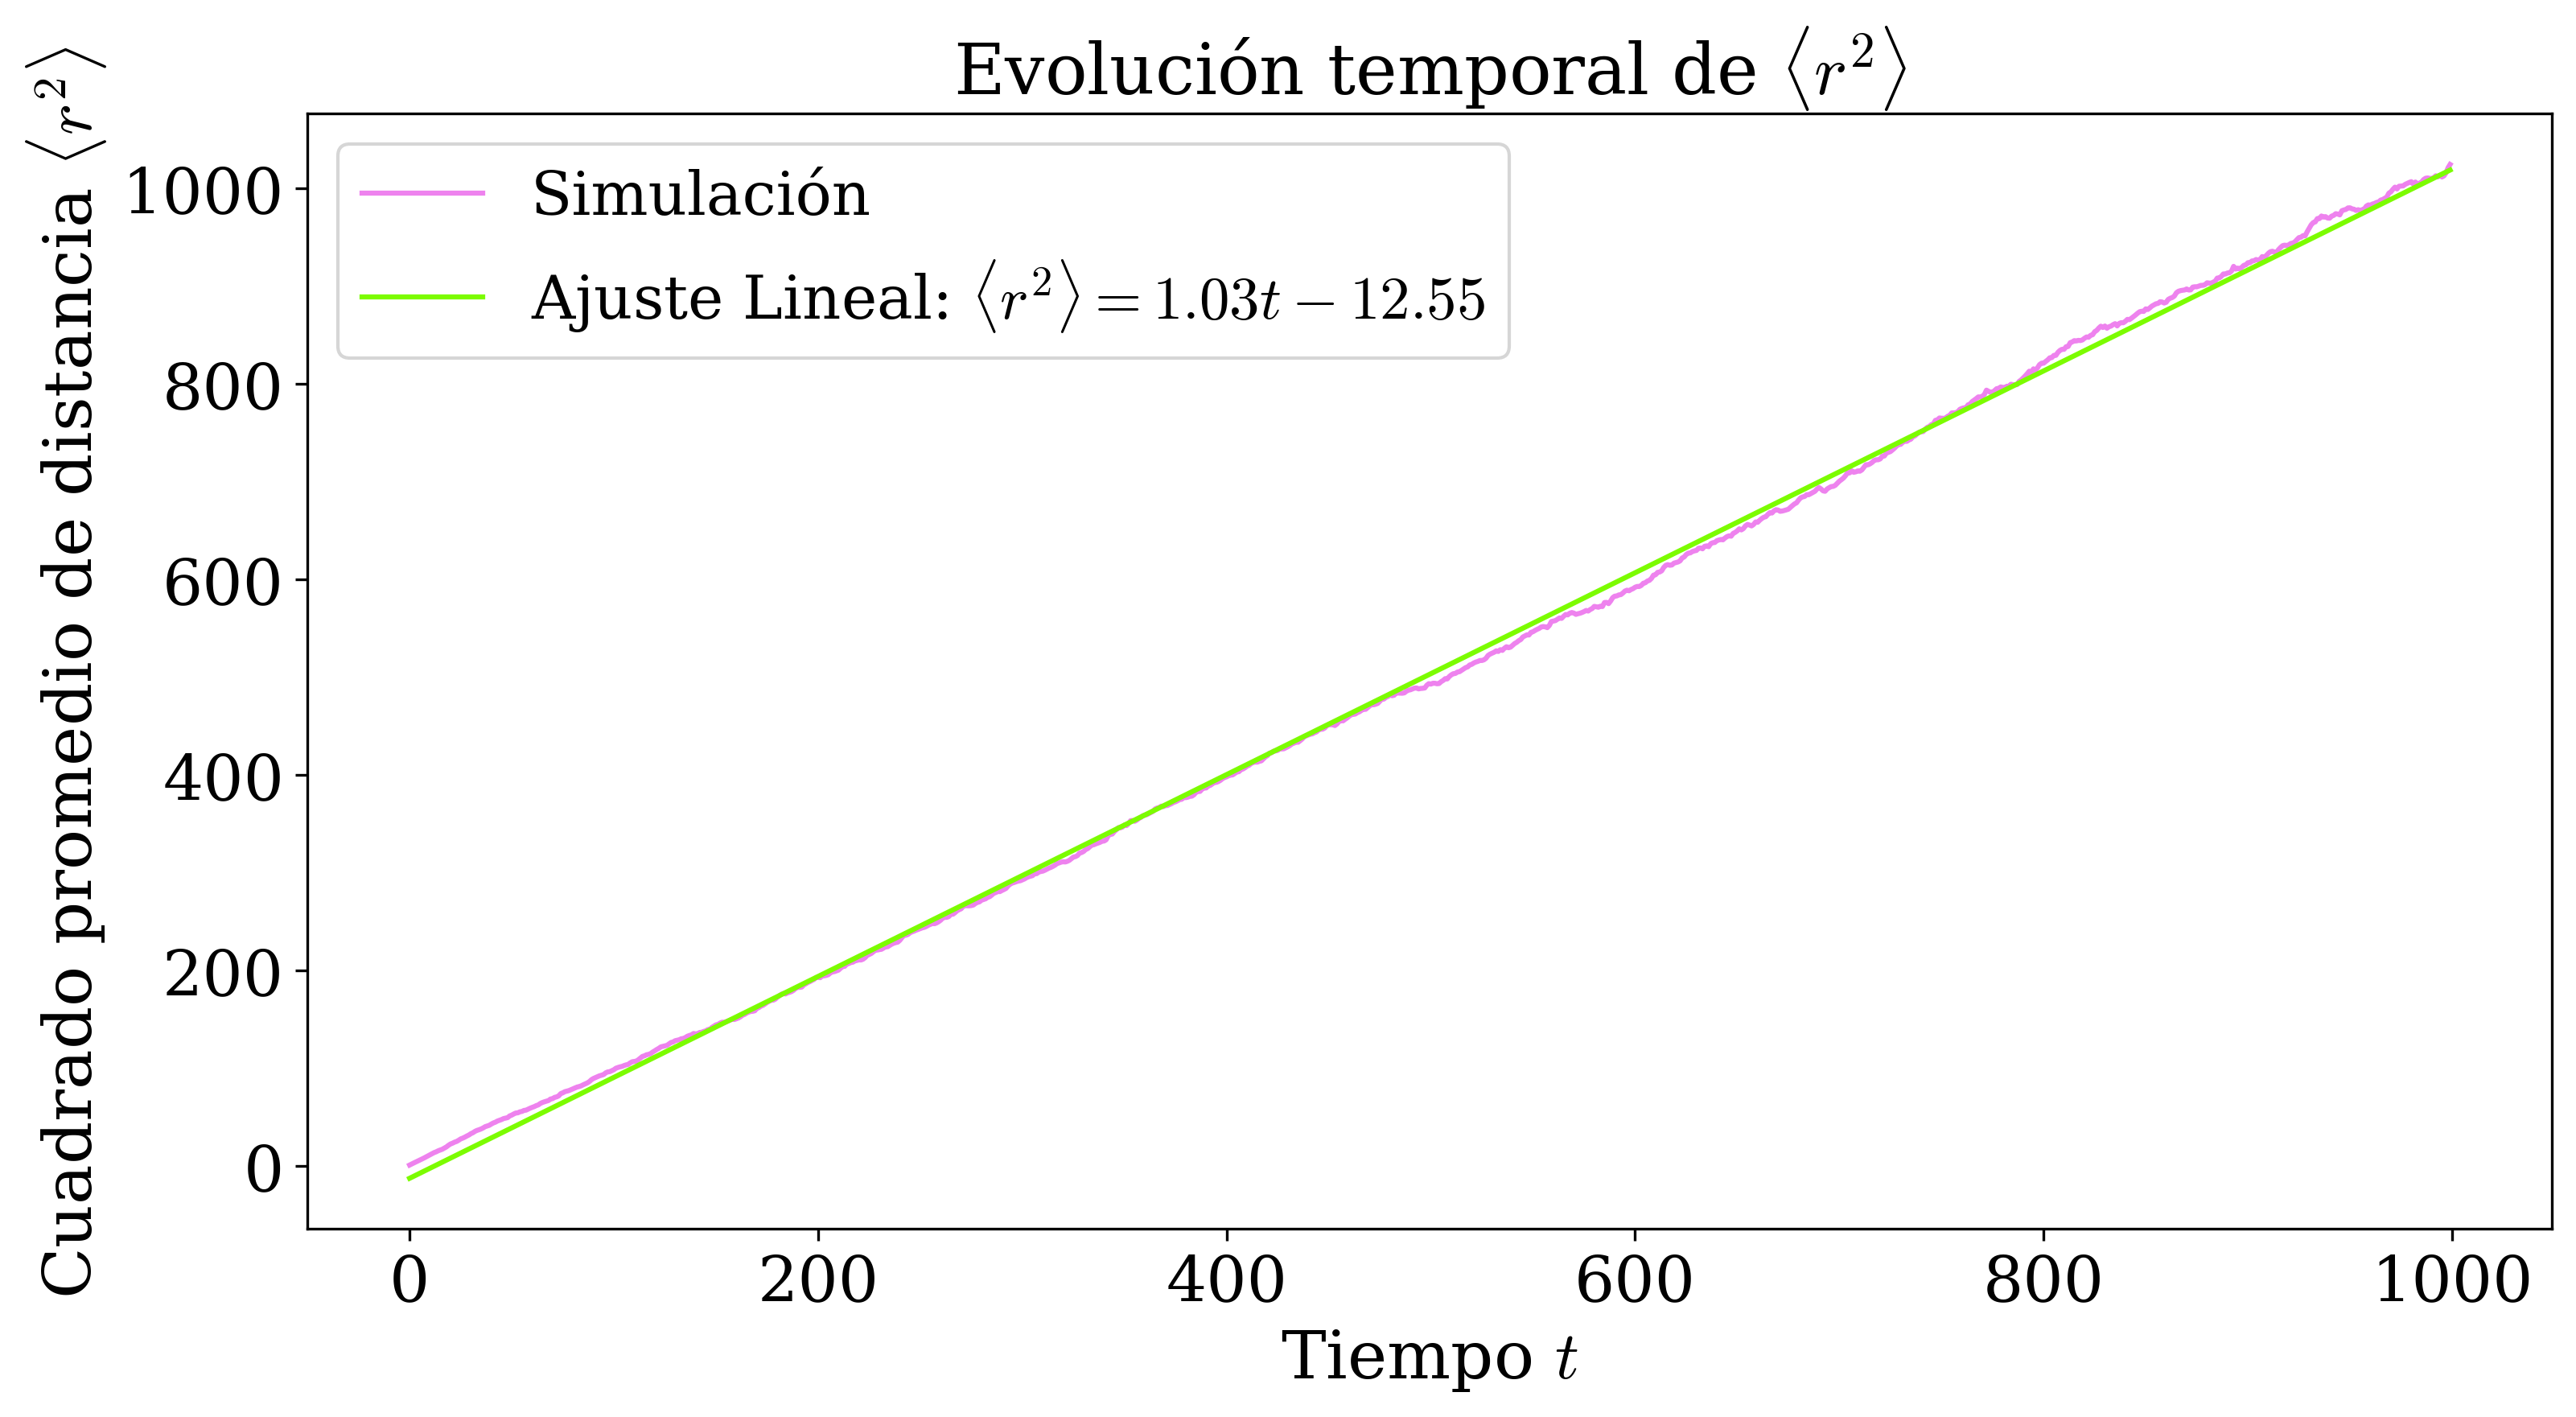
\includegraphics[width=\textwidth]{figures_tex/rw_2d_ev_cart.png}
        \caption{Ajuste lineal de $\langle r^2 \rangle$ (Cartesianas).}
        \label{fig:rw_2d_ev_cart}
    \end{minipage}
    \hfill
    \begin{minipage}{0.48\textwidth}
        \centering
        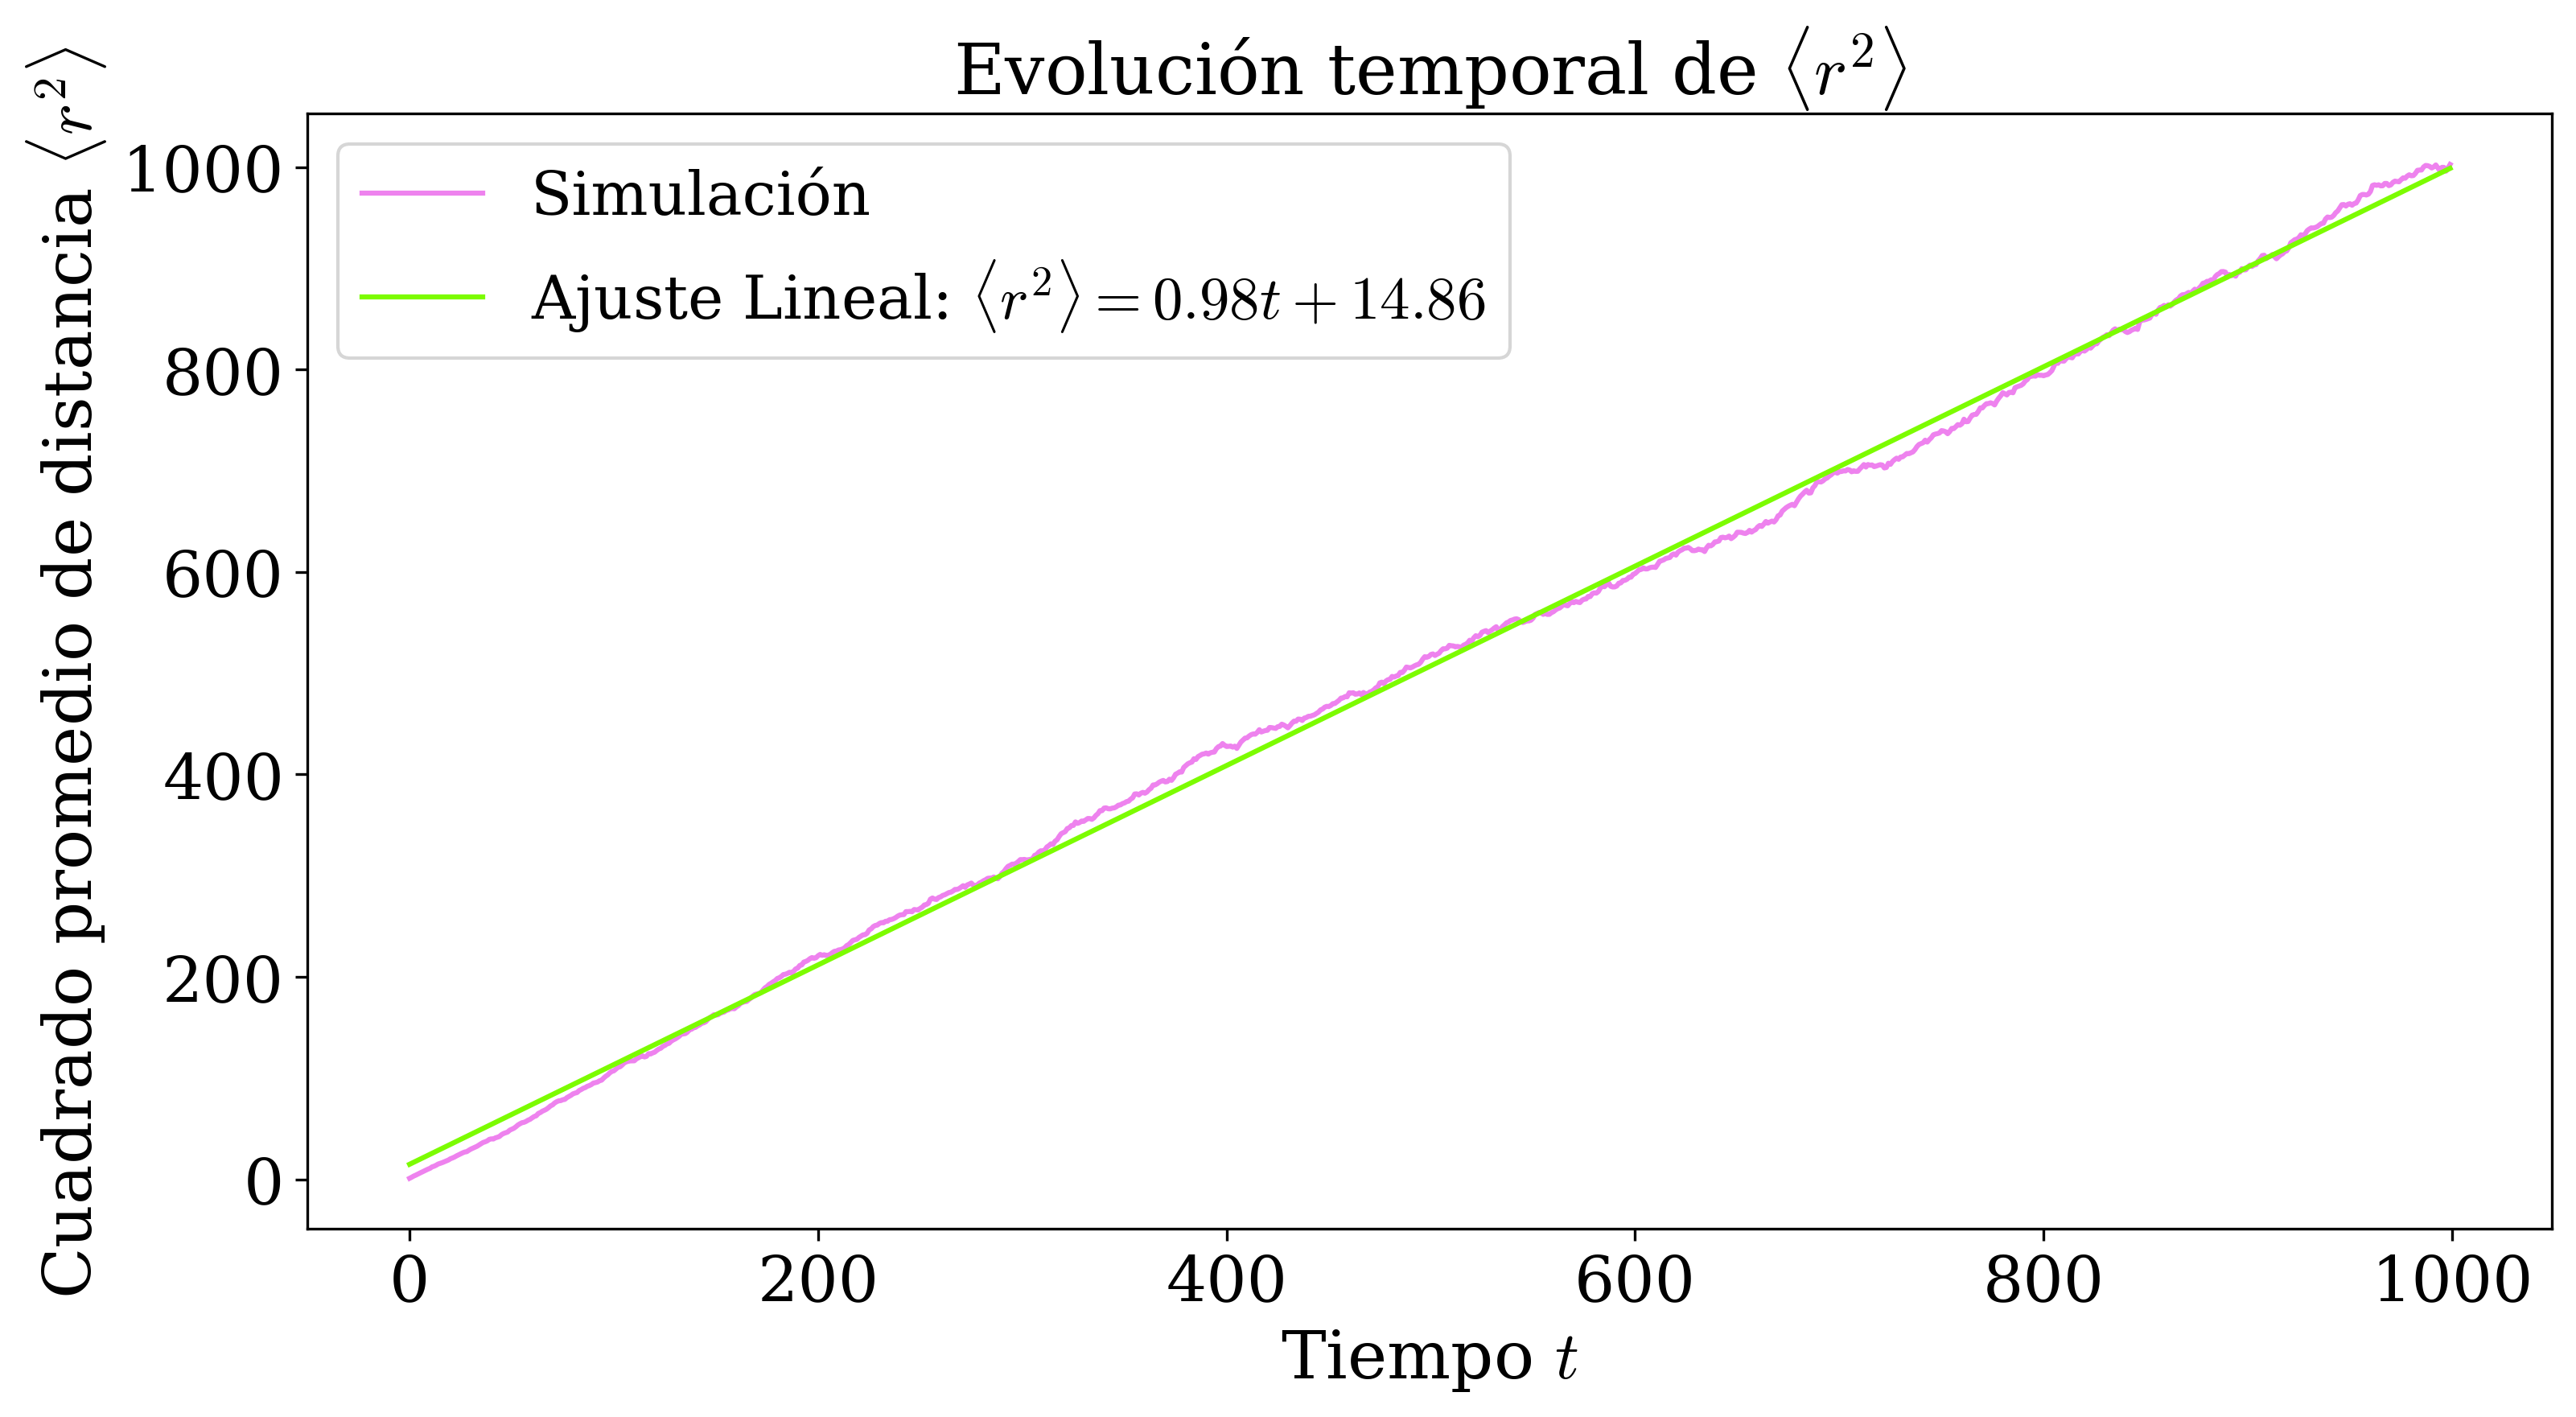
\includegraphics[width=\textwidth]{figures_tex/rw_2d_ev_polar.png}
        \caption{Ajuste lineal de $\langle r^2 \rangle$ (Polares).}
        \label{fig:rw_2d_ev_polar}
    \end{minipage}
\end{figure}

En la simulación cartesiana (Figuras \ref{fig:rw_2d_cart} y \ref{fig:rw_2d_ev_cart}) y simulación polar (Figuras \ref{fig:rw_2d_polar} y \ref{fig:rw_2d_ev_polar}) se obtiene un ajuste $\langle r^2 \rangle = 1.03t - 12.55$ y $\langle r^2 \rangle = 0.98t + 14.86$ respectivamente. Las pequeñas variaciones en la ordenada al origen y la desviación de la pendiente unitaria exacta (errores del orden de $\approx 2-3\%$) son atribuibles a fluctuaciones estadísticas debido a un tamaño de muestra $N$ finito.


\subsubsection{Caminata Aleatoria en 3D}

La expansión del modelo al espacio tridimensional se evaluó con $N=1000$ caminantes, aunque se minimizó la densidad de trayectorias para preservar la legibilidad visual del caos espacial en la Figura \ref{fig:rw_3d}.

\begin{figure}[htbp]
    \centering
    \begin{minipage}{0.48\textwidth}
        \centering
        \href{https://youtu.be/5WDNcmlZvWc?list=PLYDzV8MgIoON7YU9Pd_x0HvjzlLKixw87}{
        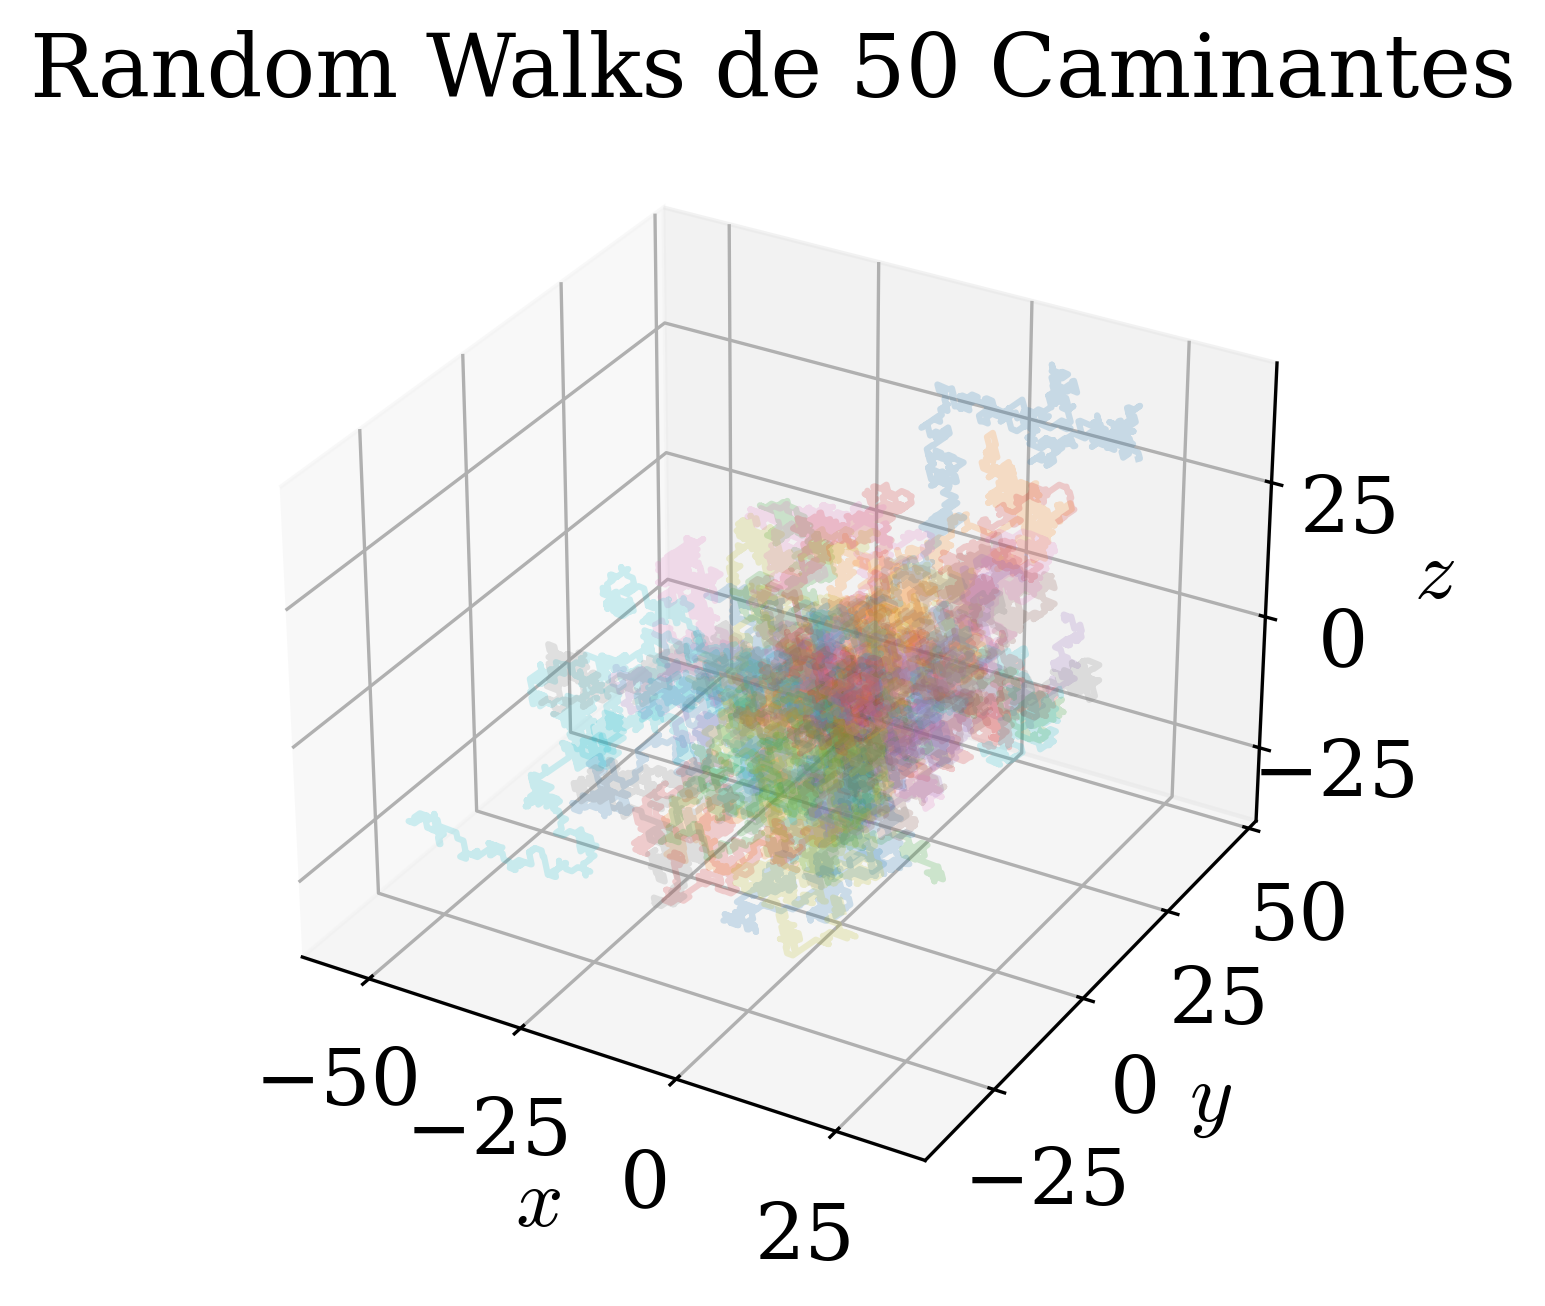
\includegraphics[width=\textwidth]{figures_tex/rw_3d.png}}
        \caption{Trayectorias espaciales ($x,y,z$).}
        \label{fig:rw_3d}
    \end{minipage}\hfill
    \begin{minipage}{0.48\textwidth}
        \centering
        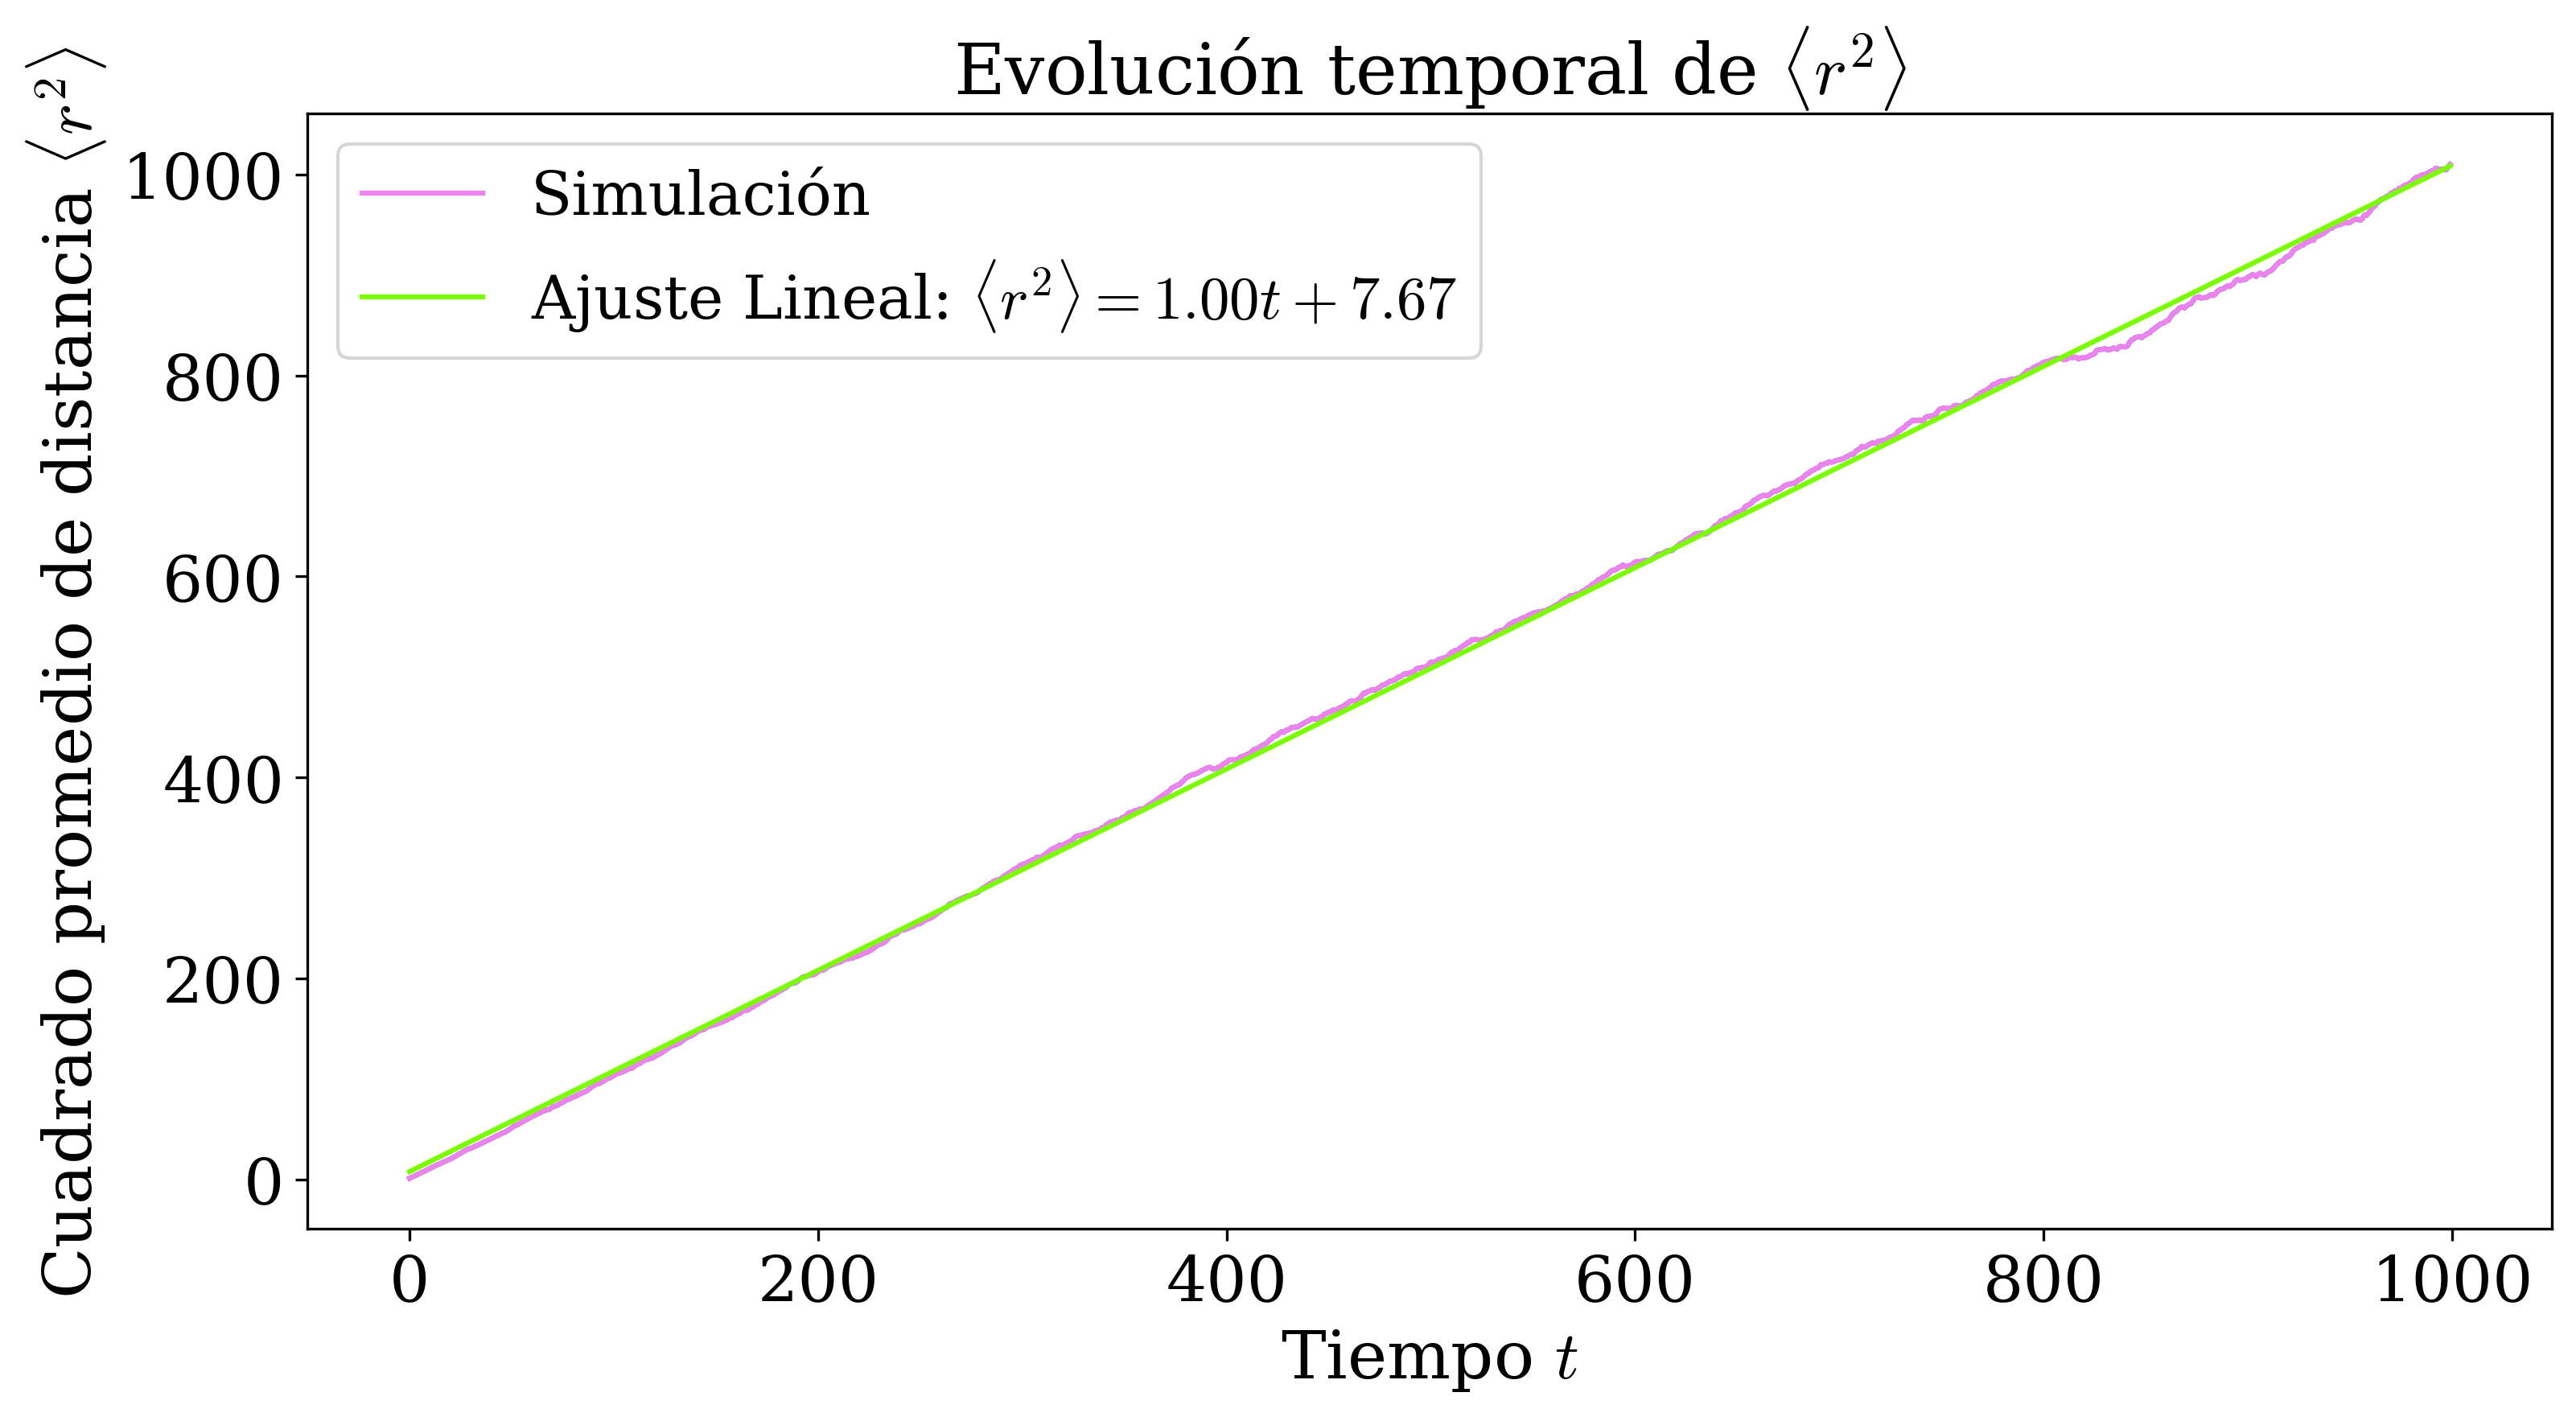
\includegraphics[width=\textwidth]{figures_tex/rw_3d_ev.png}
        \caption{Evolución temporal y ajuste lineal de $\langle r^2 \rangle$ en 3D.}
        \label{fig:rw_3d_ev}
    \end{minipage}
\end{figure}

La visualización tridimensional (Figura \ref{fig:rw_3d}) para $N=50$ agentes exhibe un agrupamiento central esférico denso con ramificaciones estocásticas hacia los extremos. En cuanto al análisis de varianza posicional (Figura \ref{fig:rw_3d_ev}), este devuelve una relación excepcionalmente precisa: $\langle r^2 \rangle = 1.00t + 7.67$.

\subsection{Dinámica de la Difusión 2D}

Para estudiar la propagación de una concentración inicial definida, se analizó el campo escalar de densidades $u(x,y,t)$ bajo el marco determinista de la ecuación de difusión y su contraparte estocástica basada en caminatas aleatorias. En particular, se estudió la evolución de la densidad con una condición inicial tipo delta de tamaño $10\times 10$ centrada en el origen, en una región de tamaño $100\times 100$ con condiciones de contorno de Neumann homogéneas.

\begin{figure}[h!]
    \centering
    \begin{minipage}{0.48\textwidth}
        \centering
        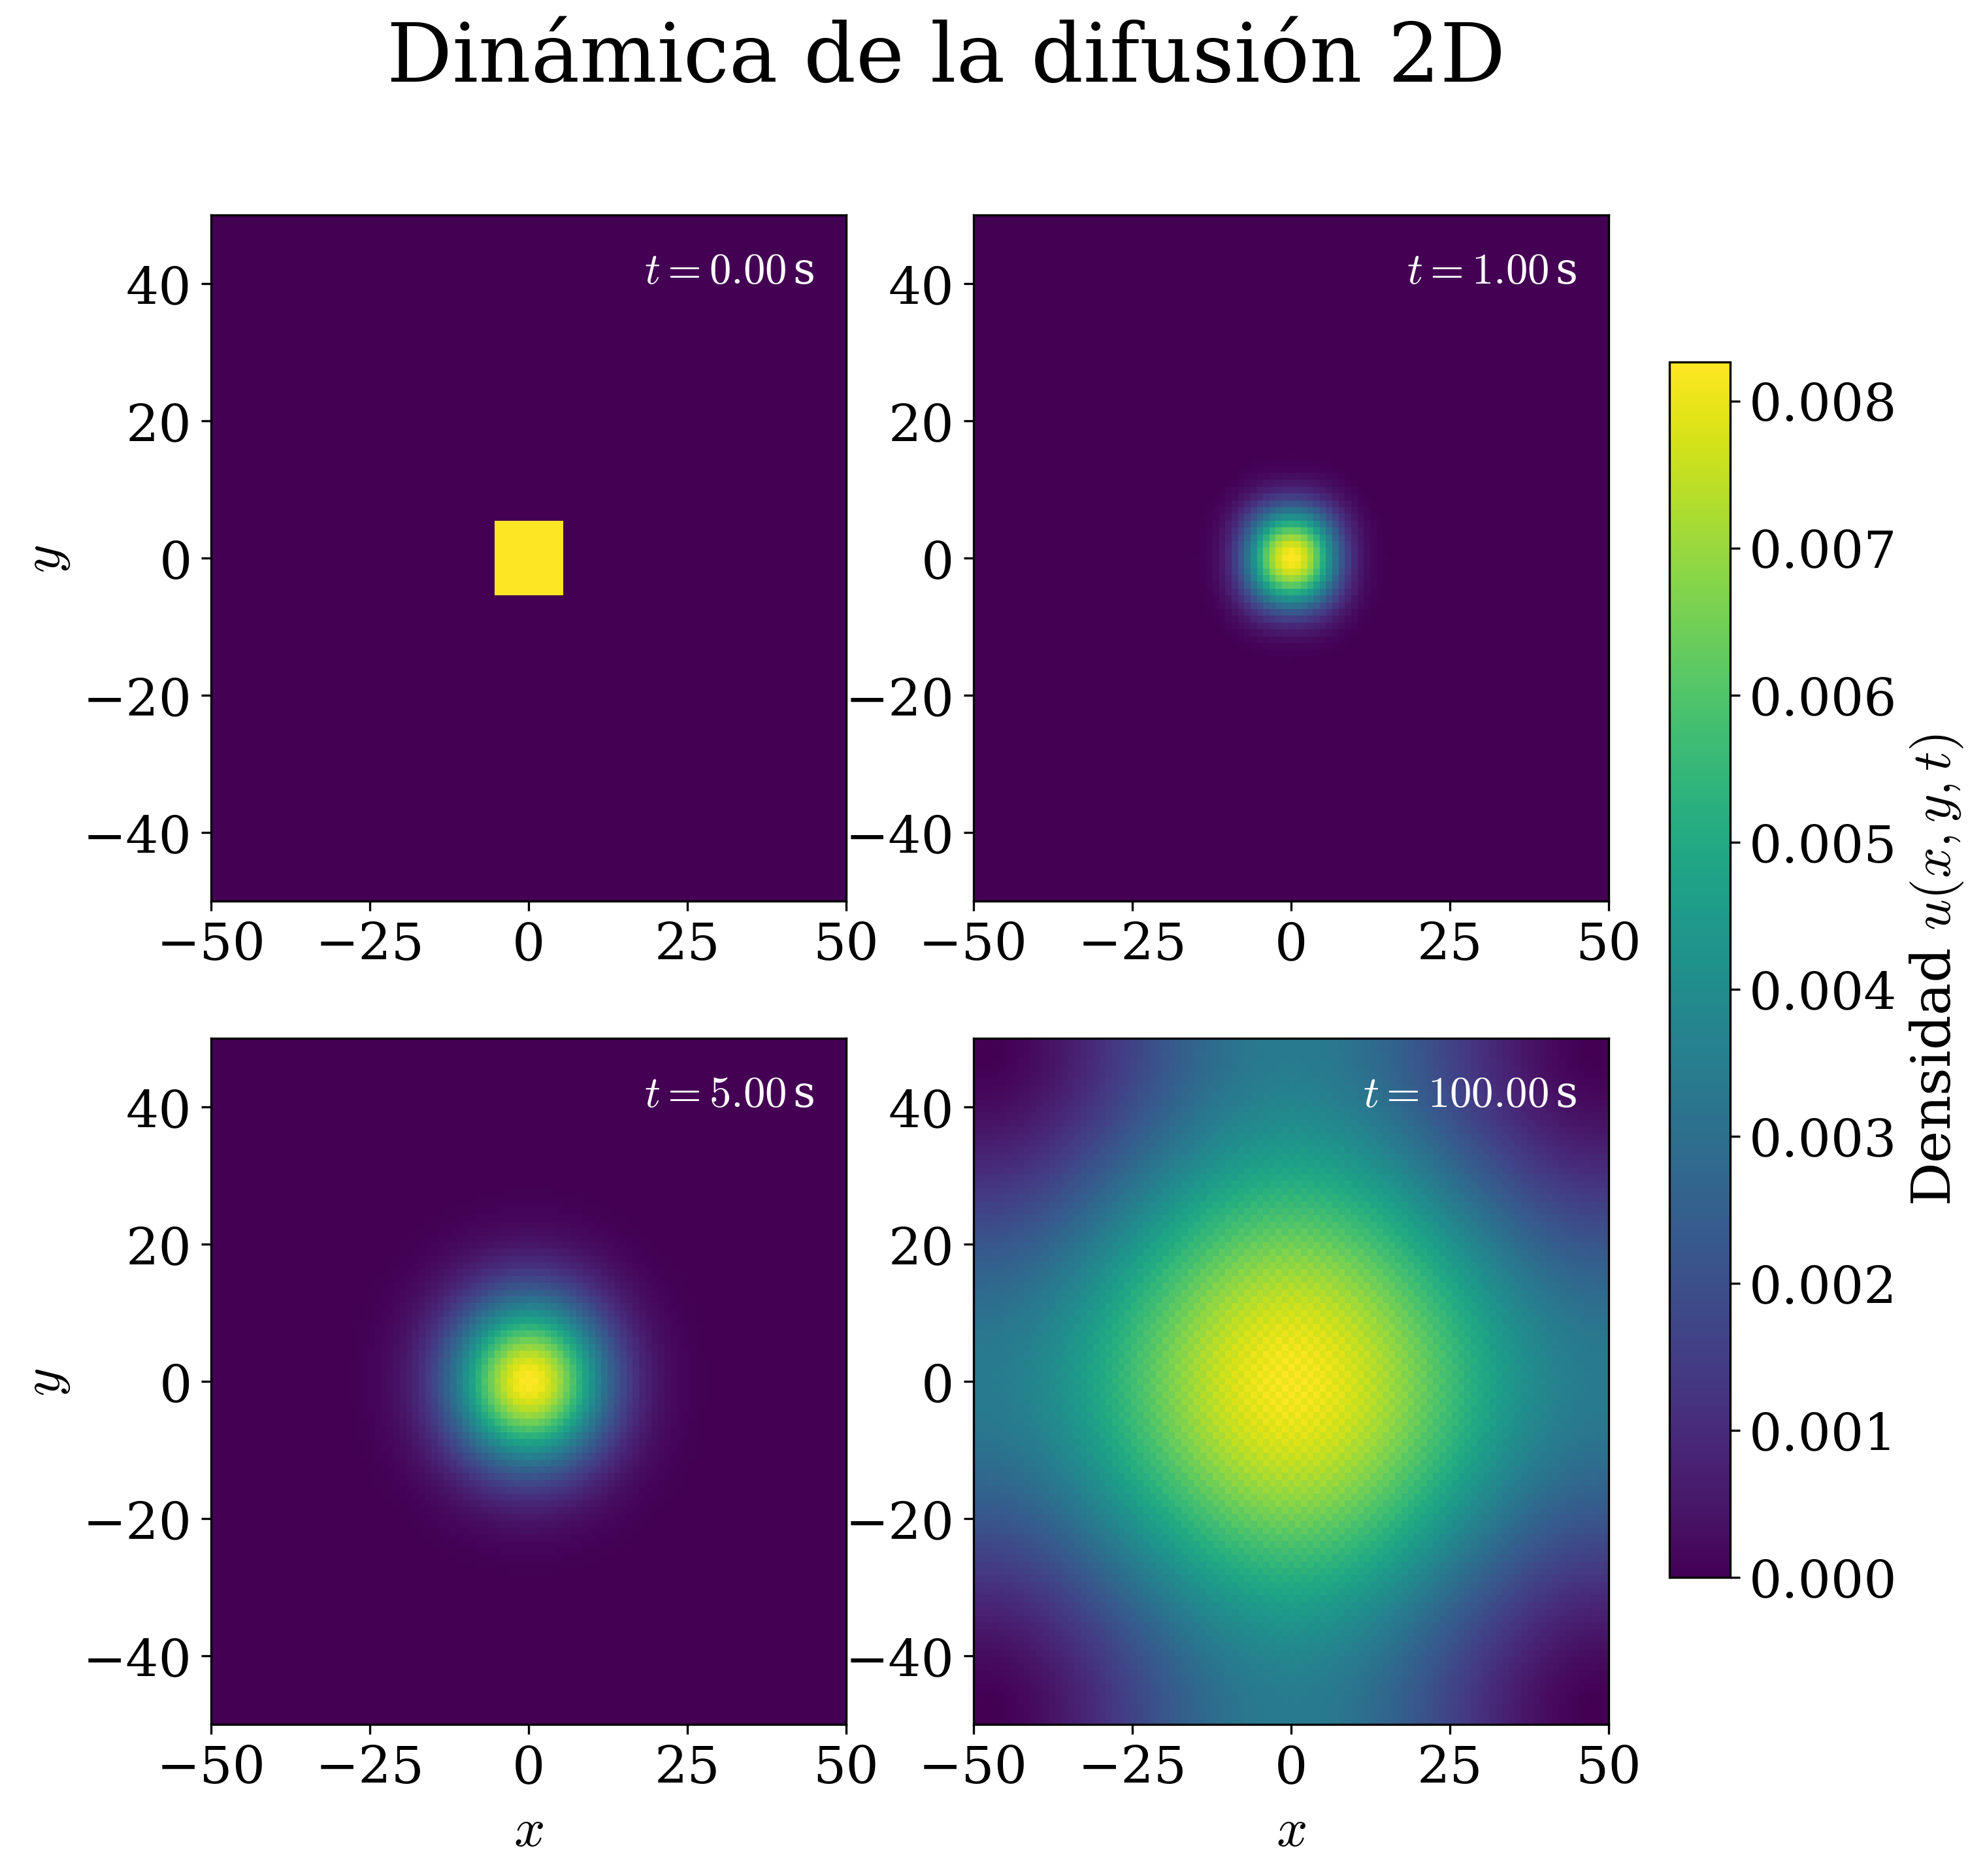
\includegraphics[width=\textwidth]{figures_tex/diffusion_cmap_determ.png}
        \caption{Evolución temporal del campo de densidad $u(x,y,t)$ mediante el modelo determinista para $t \in \{0.00, 1.00, 5.00, 100.00\}\,\text{s}$.}
        \label{fig:diff_cmap_determ}
    \end{minipage}\hfill
    \begin{minipage}{0.48\textwidth}
        \centering
        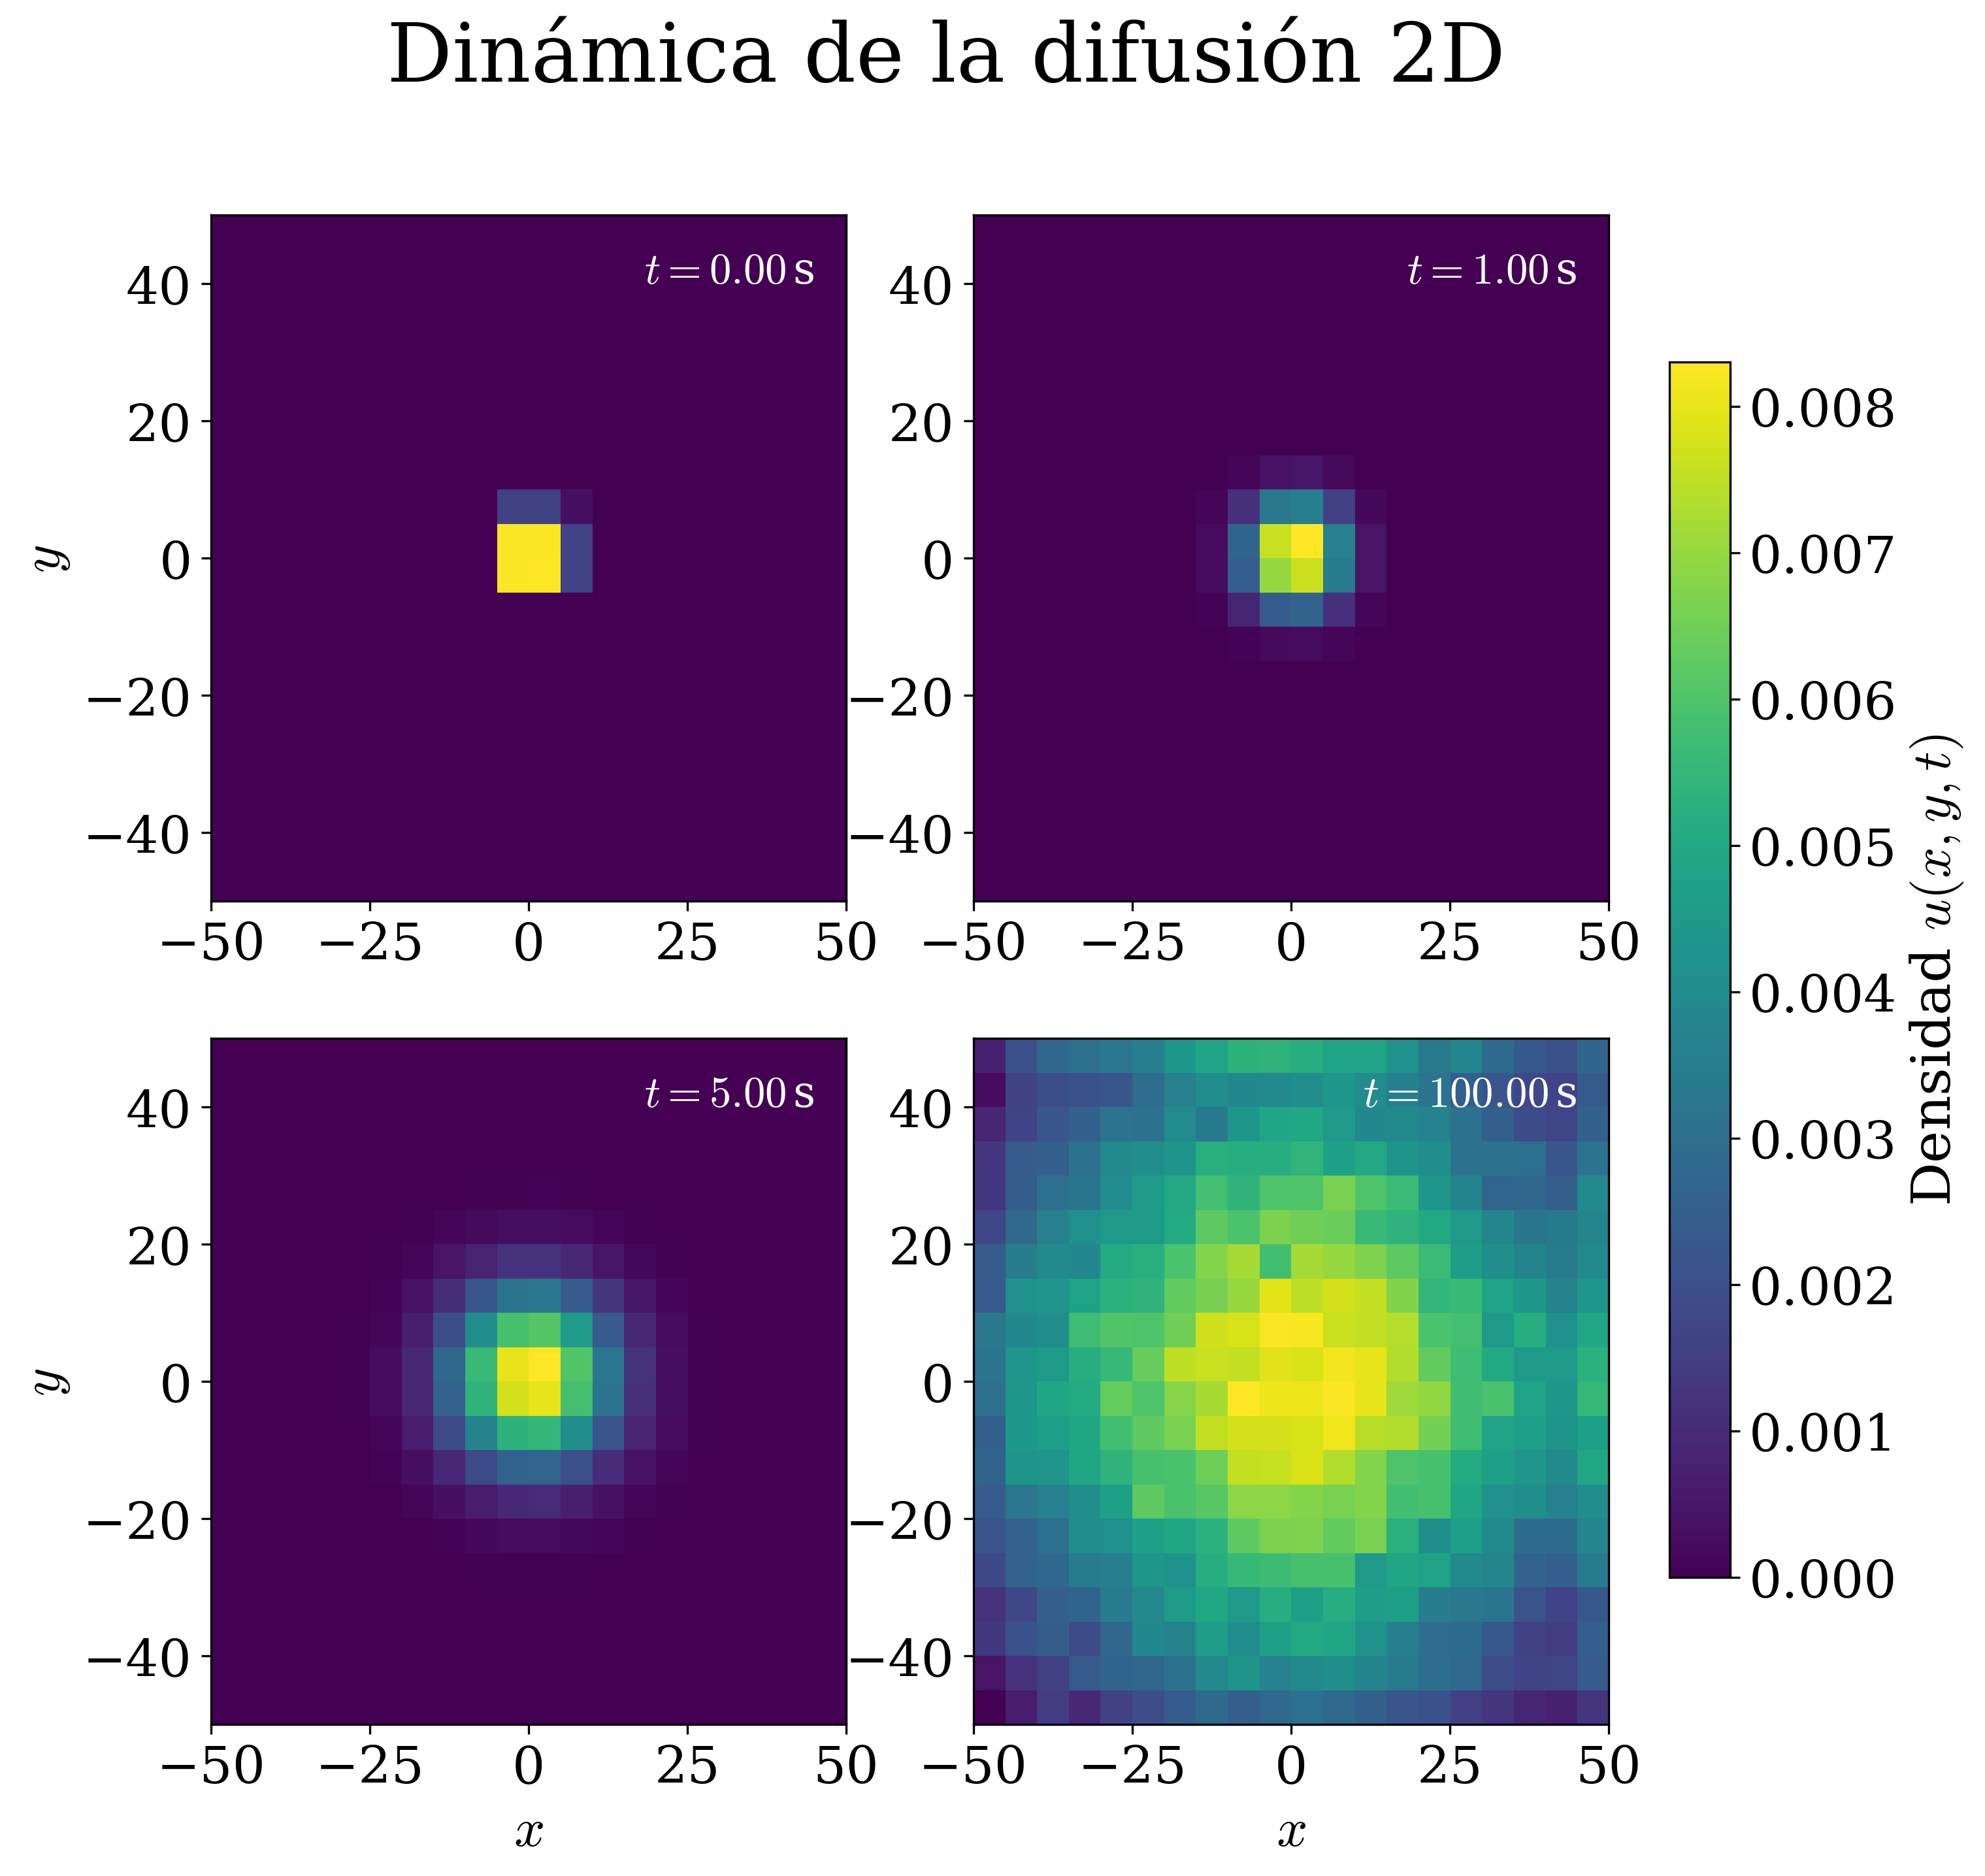
\includegraphics[width=\textwidth]{figures_tex/diffusion_cmap_rw.png}
        \caption{Evolución estocástica equivalente generada por caminadores aleatorios en un arreglo bidimensional para $t \in \{0.00, 1.00, 5.00, 100.00\}\,\text{s}$.}
        \label{fig:diff_cmap_rw}
    \end{minipage}
\end{figure}


Como ilustran las Figuras \ref{fig:diff_cmap_determ} y \ref{fig:diff_cmap_rw}, el estado inicial presenta una delta cuadrada que se ensancha monótonamente a medida que evoluciona el sistema. Dada la naturaleza de la discretización espacial en el conteo de partículas discretas, la Figura \ref{fig:diff_cmap_rw} presenta ruido de resolución, pese a exhibir el mismo patrón cualitativo. Esta congruencia entre los modelos macroscópicos continuos y estocásticos discretos evidencia que el límite macroscópico de múltiples caminatas aleatorias microscópicas es idéntico a la dinámica difusiva clásica. La Figura \ref{fig:diff_3d} aporta una visión tridimensional de la evolución de la densidad observándose un progreso que sigue una distribución gaussiana.

\begin{figure}[h!]
    \centering
        \centering
        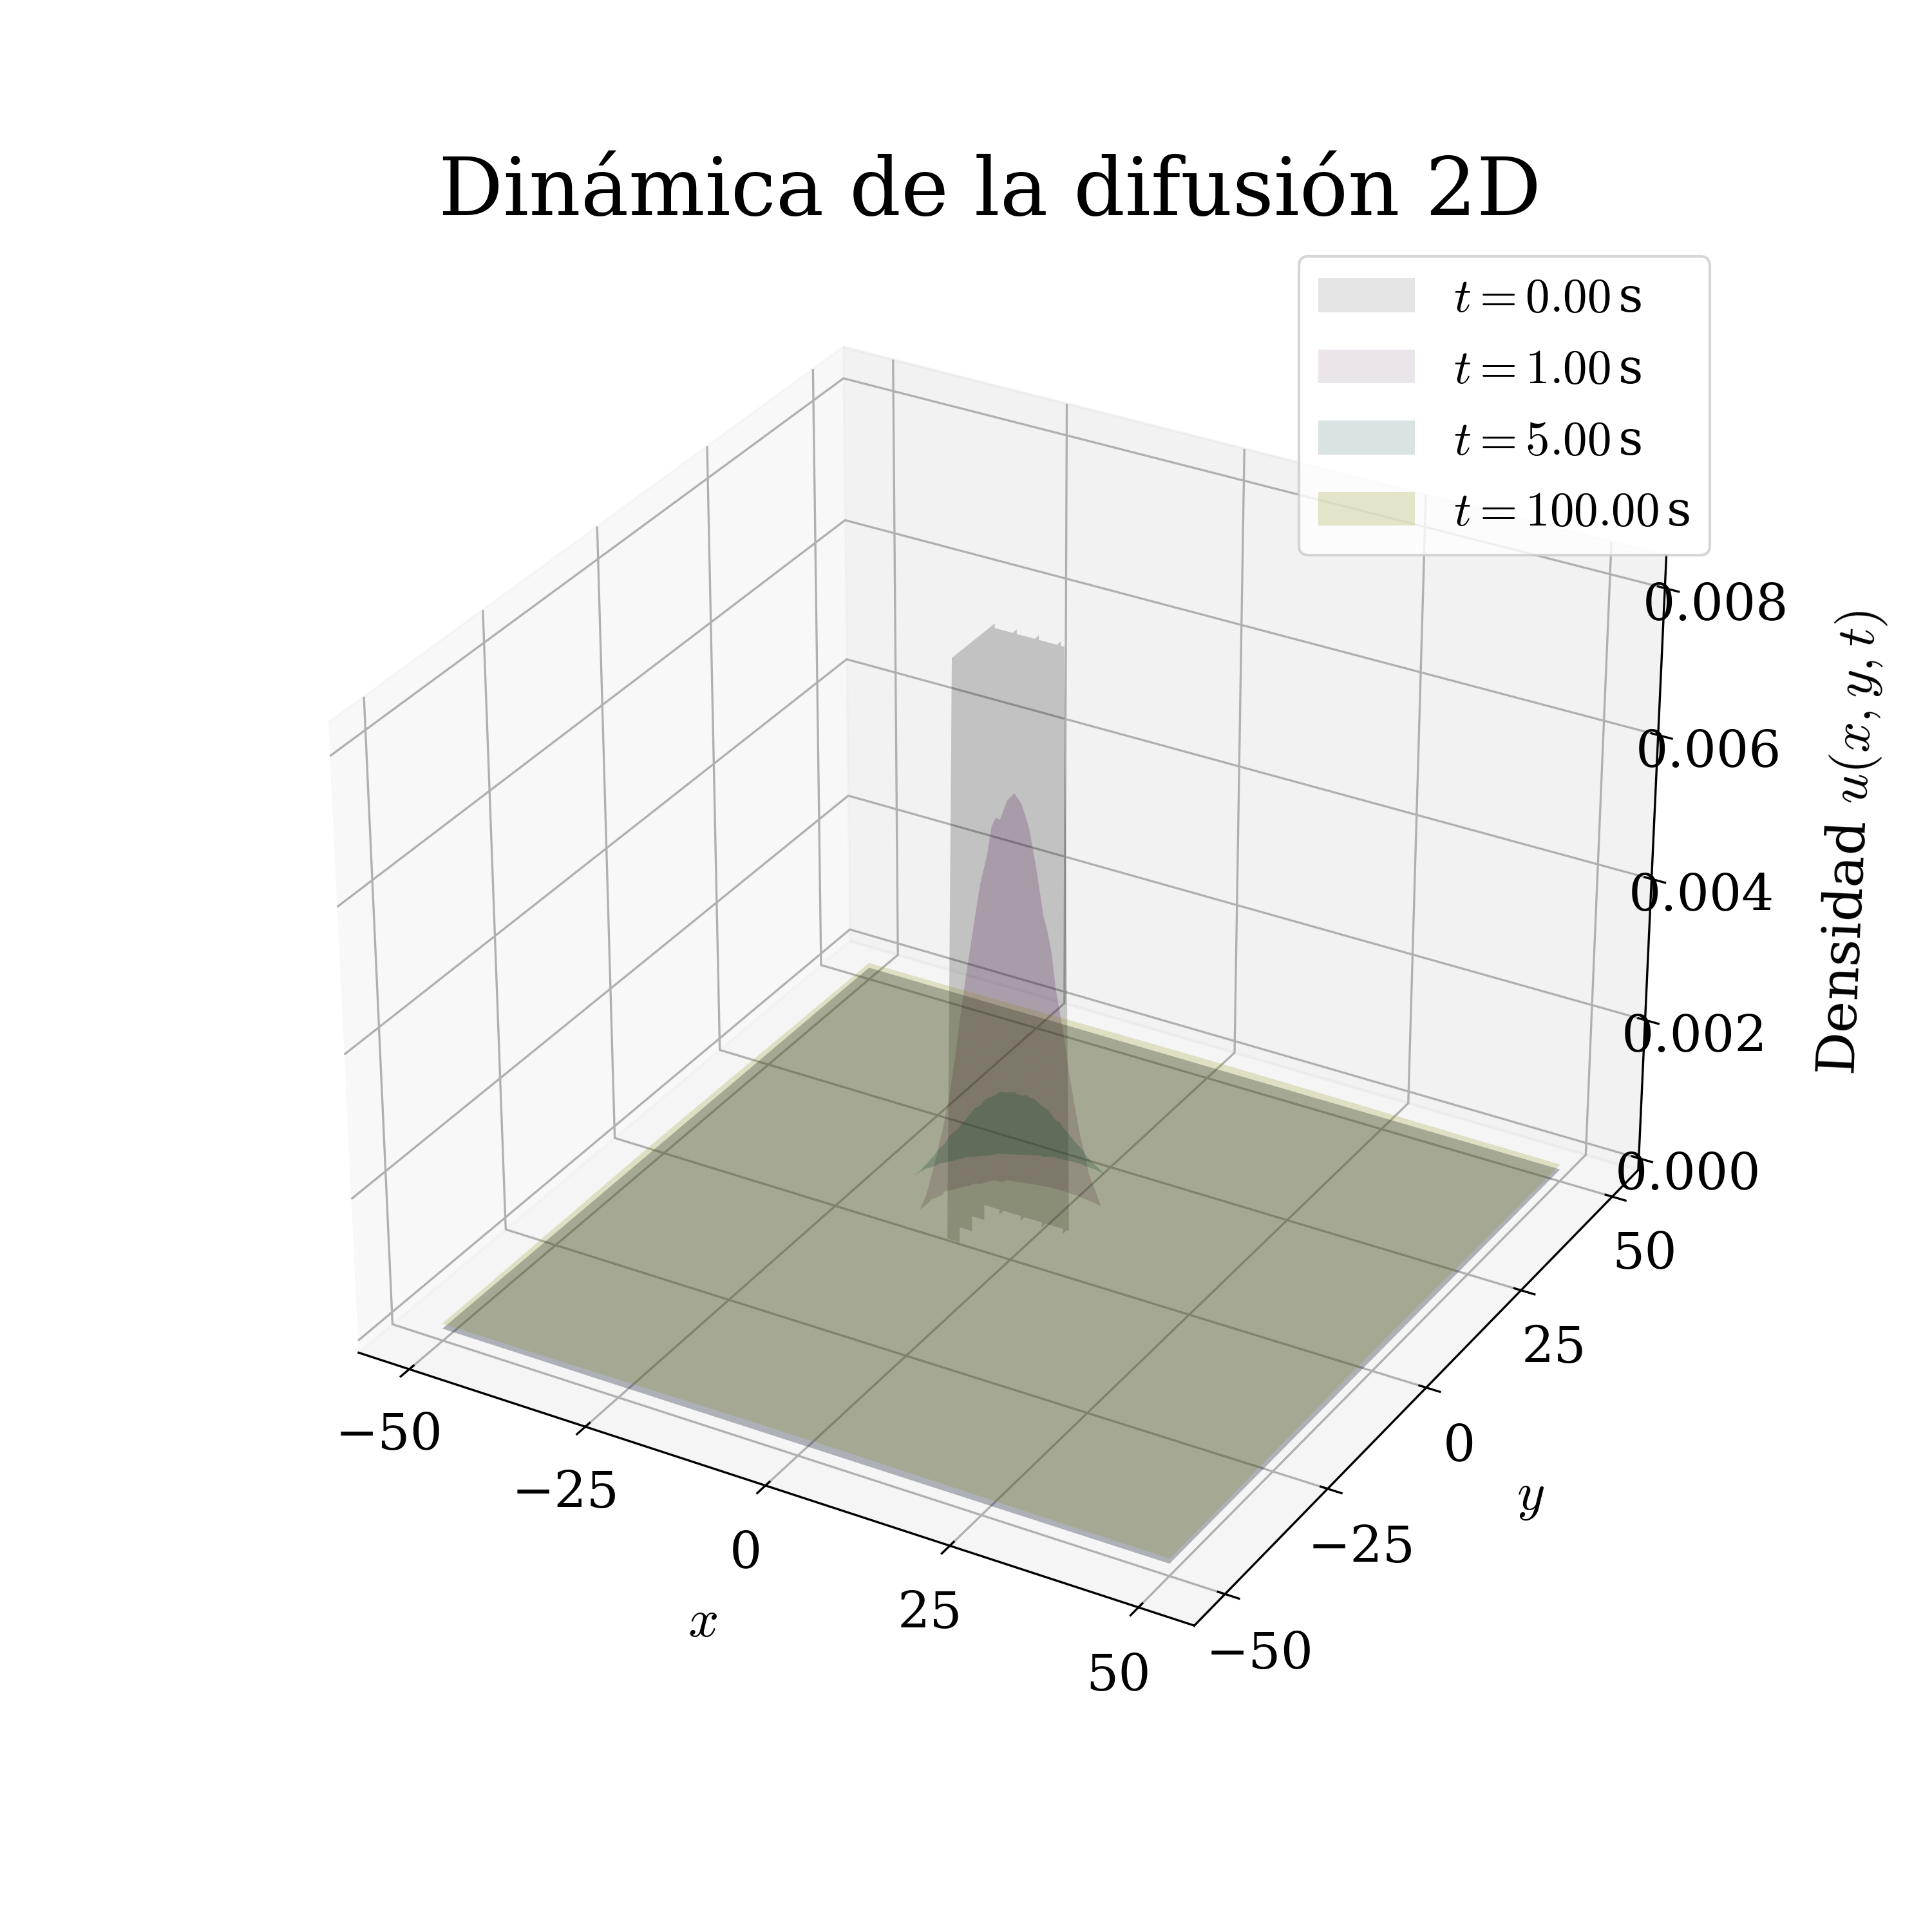
\includegraphics[width=0.5\textwidth]{figures_tex/diffusion_3d_determ.png}
        \caption{Superficie 3D de la densidad de probabilidad difusiva para el modelo determinista.}
        \label{fig:diff_3d}
\end{figure}

Adicionalmente, se realizó un estudio de la evolución entrópica en función del tamaño del dominio. Independientemente del tamaño, este análisis entrópico muestra una fase de crecimiento rápida seguida de una saturación asintótica correspondiente al estado de máximo mezclado. La regresión aplicada a los distintos tamaños del dominio corrobora la relación empírica de escalamiento termodinámico $t_{\rm eq} \propto L^2$, con $t_{\rm eq}$ el tiempo en el cual se tiene una saturación del $95\%$.


\begin{figure}[h!]
    \centering
    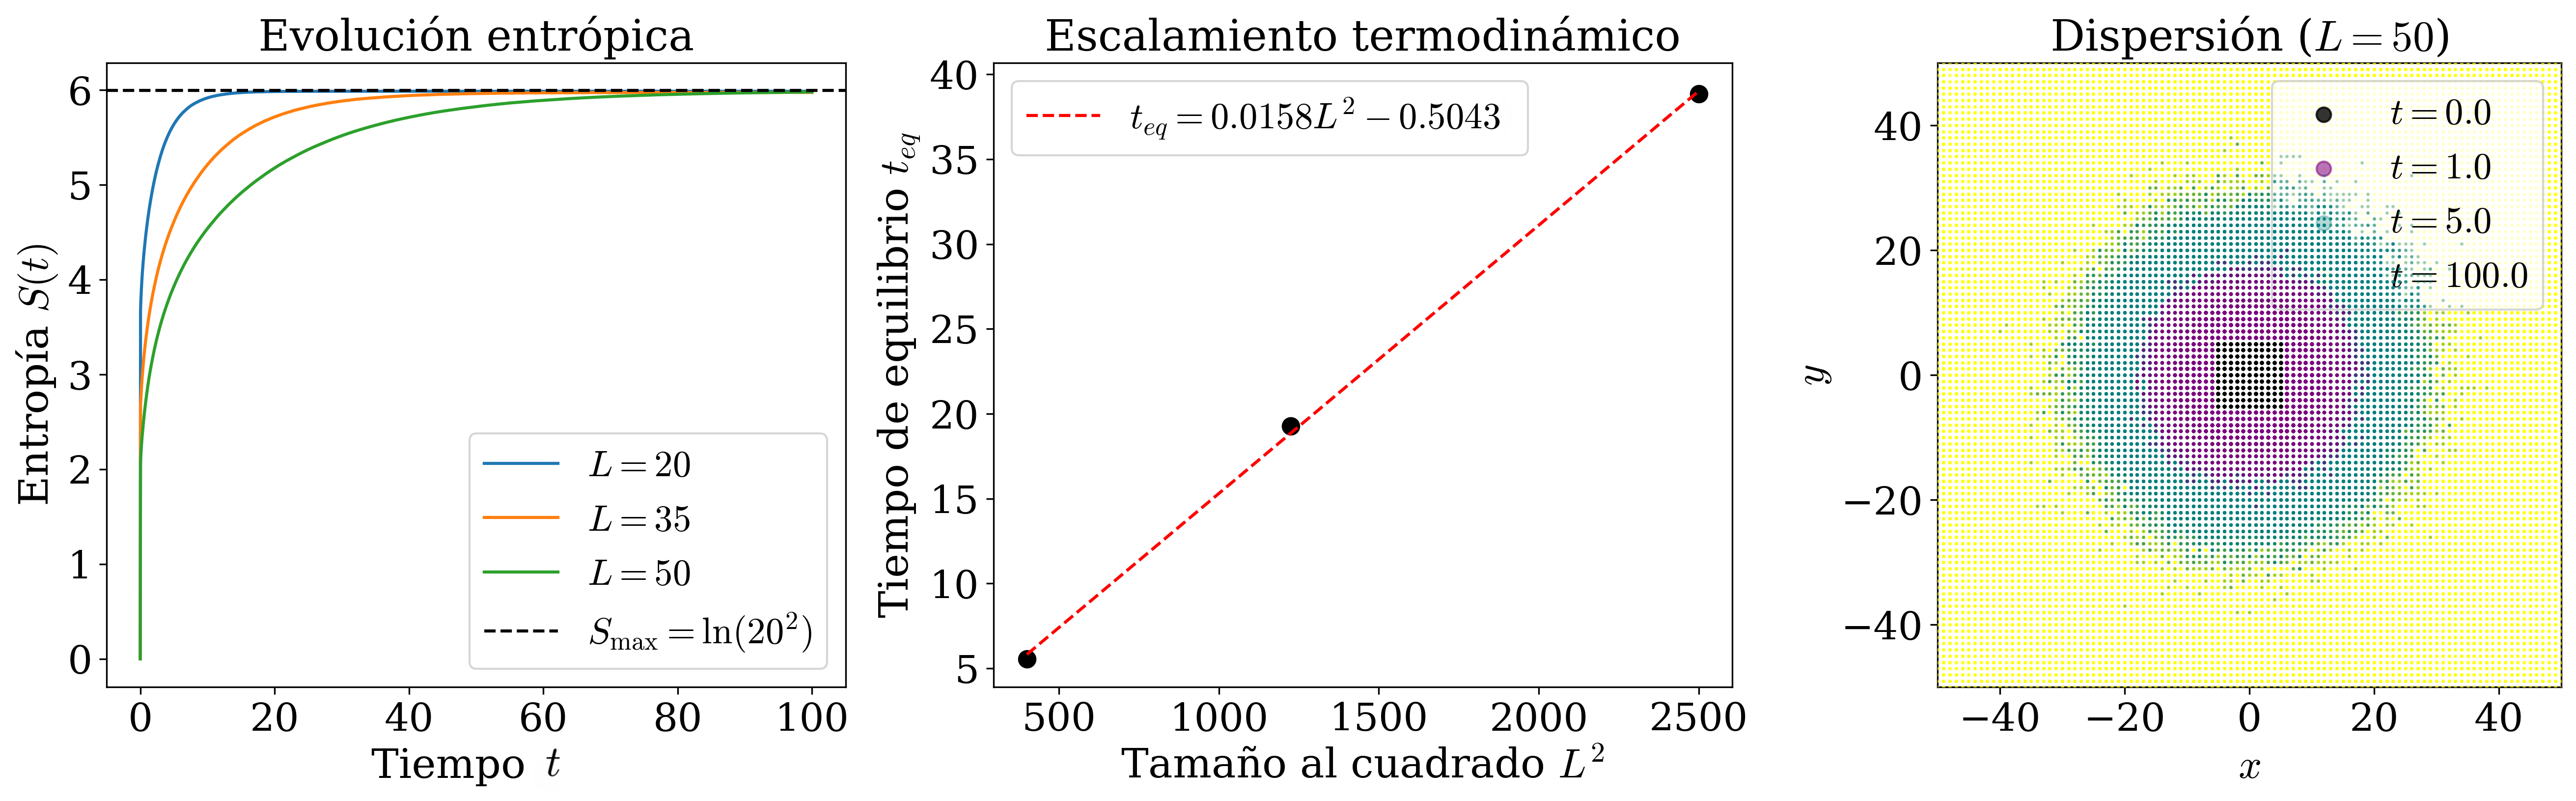
\includegraphics[width=\textwidth]{figures_tex/multiplot_analysis_rw.png}
    \caption{A la izquierda: Evolución de la entropía $S(t)$ hacia el equilibrio macroscópico. Centro: Ajuste lineal del tiempo de relajación frente a $L^2$. Derecha: Dispersión acumulada para $L=50$.}
    \label{fig:entropy_scaling}
\end{figure}

\newpage

\subsection{Percolación}


Por último, el algoritmo de percolación de invasión reproduce satisfactoriamente el crecimiento fractal del fluido invasor. En la Figura \ref{fig:percolation} se muestra la matriz reticular con el mapa de resistencias (ruido blanco subyacente) sobre el que se encuentra el cluster resultante. Es notable cómo la fase invasora rodea regiones de alta resistencia, dejando zonas sin invadir (\textit{trapped regions}) y canalizándose a través de los caminos de menor energía, capturando la esencia física de la capilaridad en un medio poroso.
La aparición de este \textit{spanning cluster} (cúmulo expandido) evidencia que la densidad de probabilidad ocupacional del sistema ($p$) ha cruzado el umbral crítico de percolación ($p_c$). La marcada rugosidad del contorno y los ramales sin salida (\textit{dead ends}) confieren al cúmulo una dimensión fractal $D_f < 2$. En términos de física de transporte, este es un estado de transición de fase de segundo orden crítico; un caminante aleatorio inyectado en este régimen dejaría de exhibir difusión isotrópica regular y transicionaría a un transporte anómalo a través del laberinto fractal de caminos percolantes.


\begin{figure}[htbp]
    \centering
    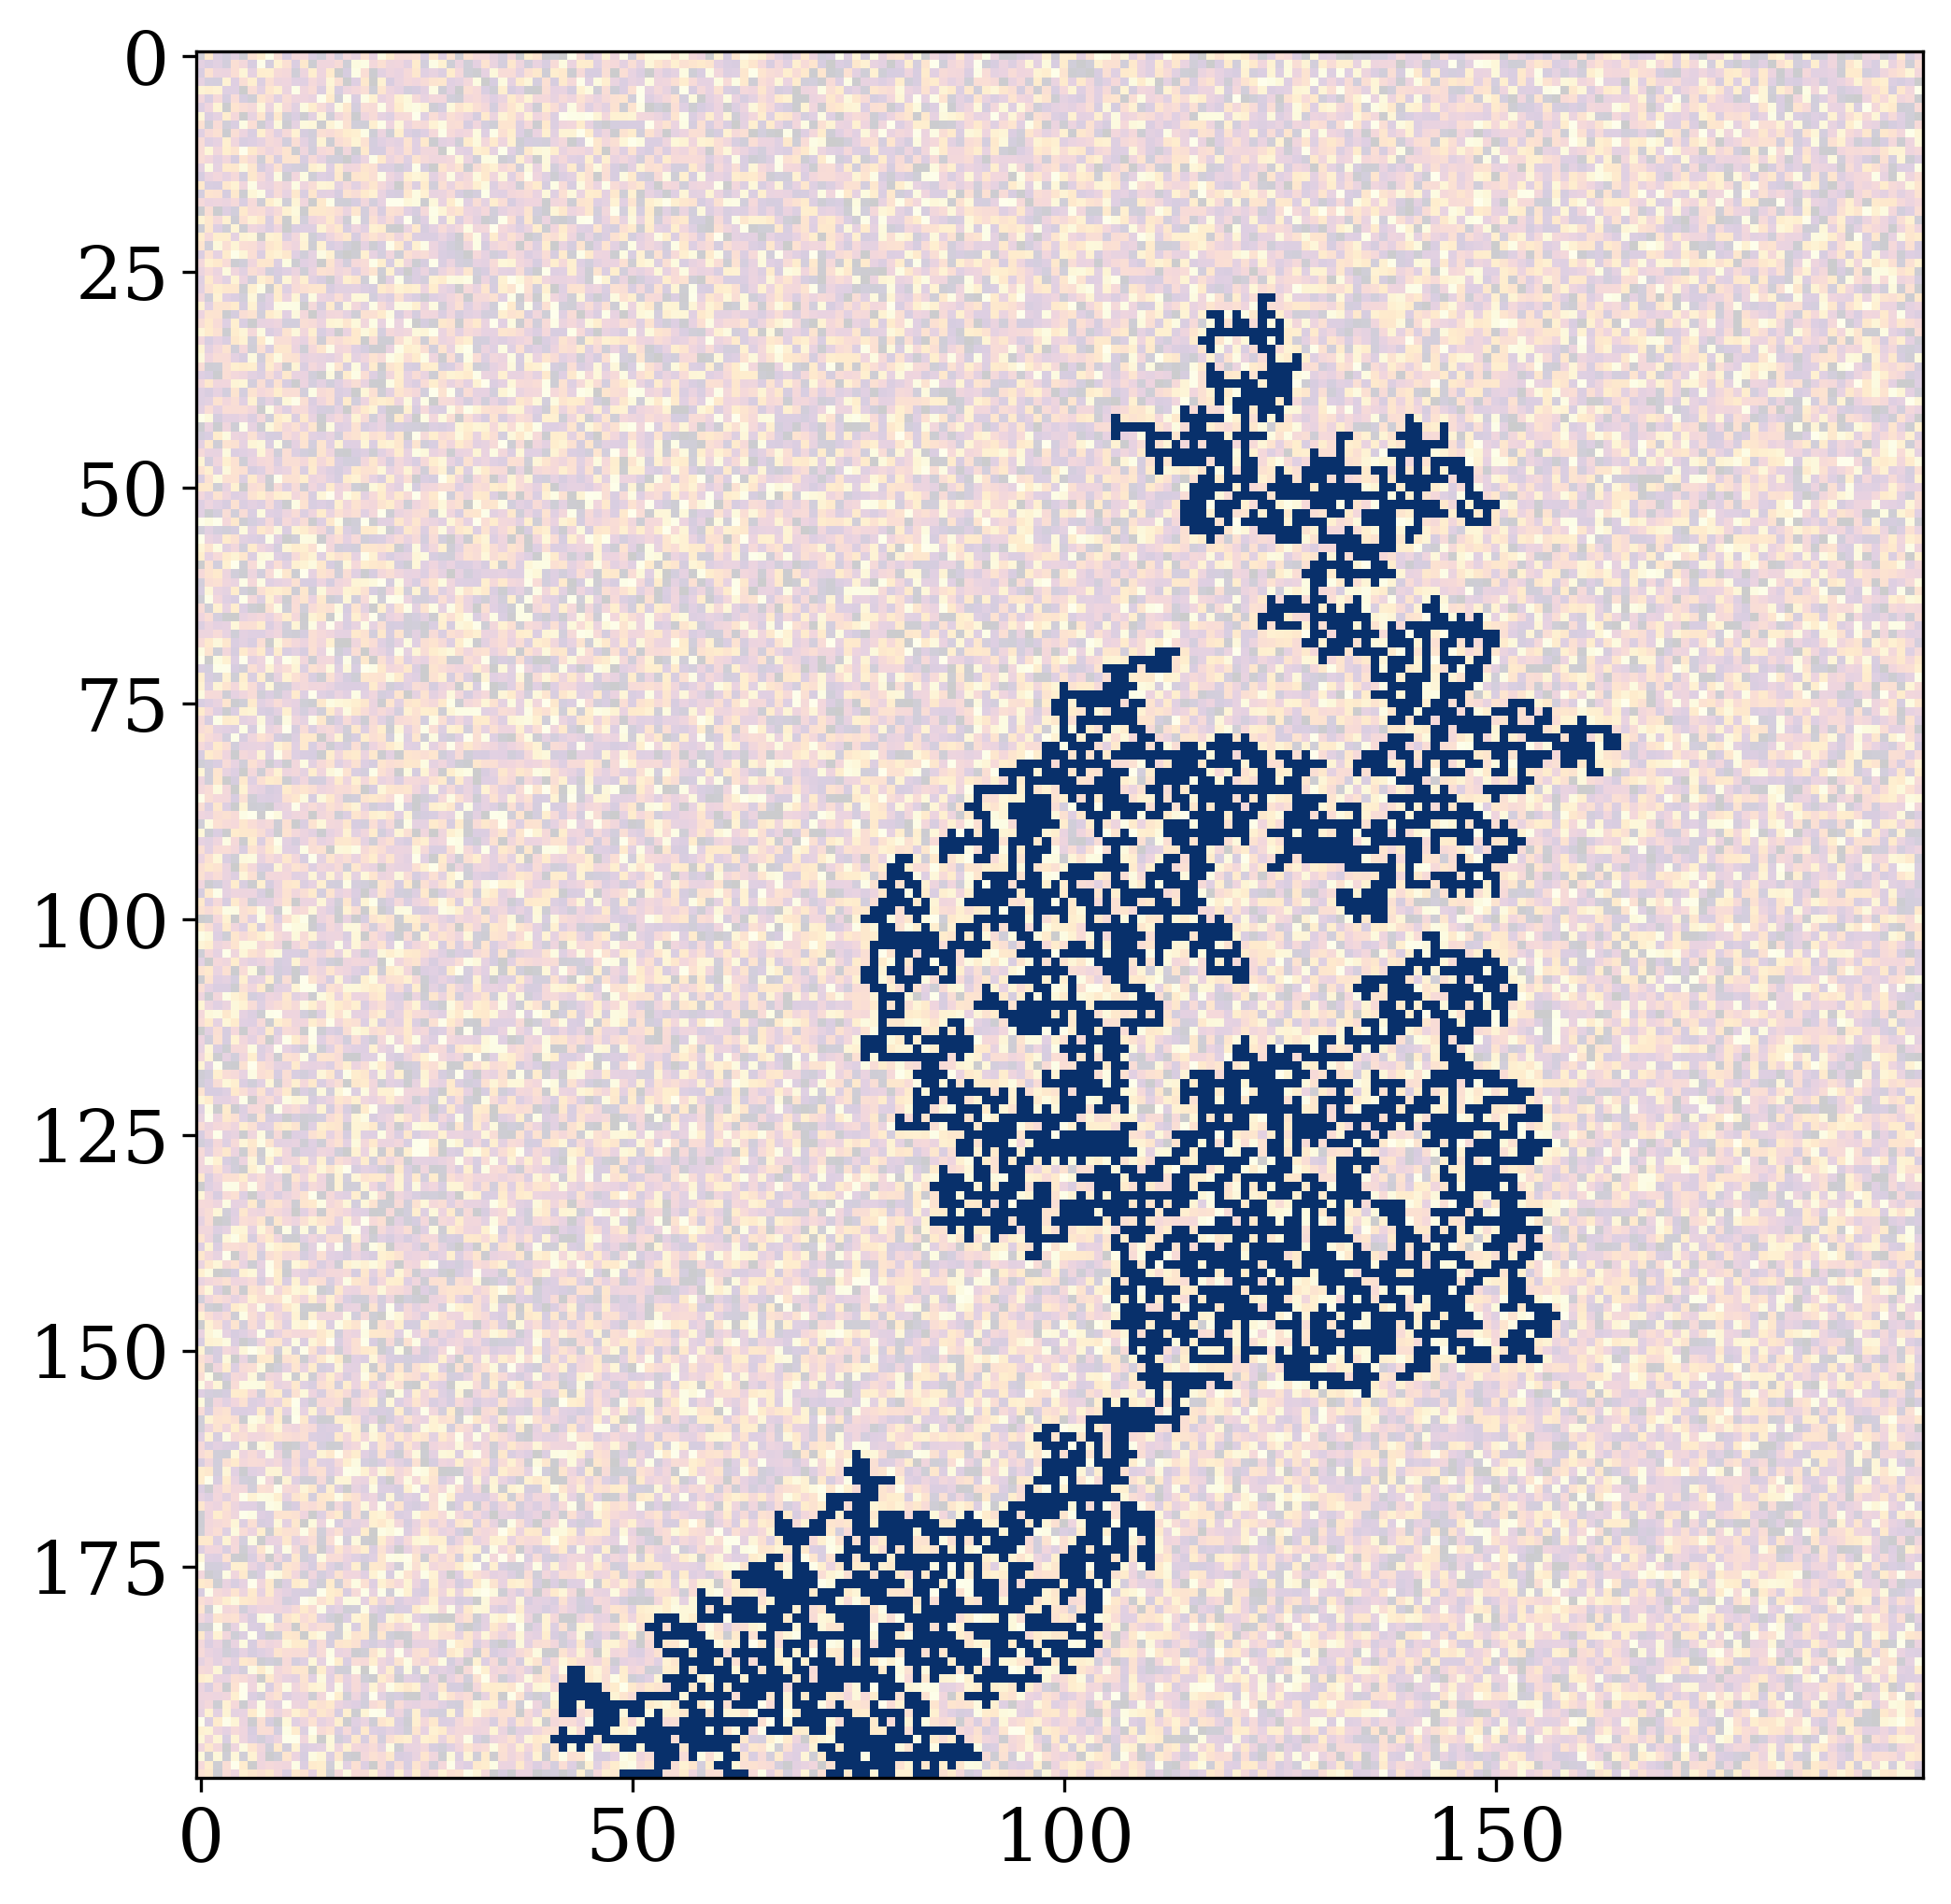
\includegraphics[width=0.6\textwidth]{figures_tex/percolation.png}
    \caption{Simulación de un cúmulo de percolación en una red bidimensional.}
    \label{fig:percolation}
\end{figure}

